\documentclass[journal]{IEEEtran}

\usepackage{adjustbox}
\usepackage{algorithm}
\usepackage{algpseudocode}
\usepackage{amsfonts}
\usepackage{amsmath}
\usepackage{amssymb}
\usepackage{amsthm}
\usepackage{bookmark}
\usepackage[american]{circuitikz}
\usepackage{cite}
\usepackage{fixmath}
\usepackage[acronym]{glossaries-extra}
\usepackage{hyperref}
\usepackage{import}
\usepackage{mathtools}
\usepackage{microtype}
\usepackage[short]{optidef}
\usepackage{pgfplots}
\usepackage[subtle]{savetrees}
\usepackage{siunitx}
\usepackage{stfloats}
\usepackage[caption=false,font=footnotesize,subrefformat=parens,labelformat=parens]{subfig}
\usepackage{tikz}
\usepackage{xcolor}

% dark mode
\usepackage{xcolor} \pagecolor[rgb]{0,0,0} \color[rgb]{1,1,1}

% amsthm
\newtheorem{proposition}{Proposition}
\newtheorem{remark}{Remark}

% siunitx
\DeclareSIUnit{\belm}{Bm}
\DeclareSIUnit{\dBm}{\deci\belm}
\DeclareSIUnit{\beli}{Bi}
\DeclareSIUnit{\dBi}{\deci\beli}

% PGF/TikZ
\usetikzlibrary{arrows,calc,matrix,patterns,plotmarks,positioning}
\usepgfplotslibrary{groupplots,patchplots}
\pgfplotsset{compat=newest}

% algpseudocode
\makeatletter
\renewcommand{\fnum@algorithm}{\fname@algorithm{} \thealgorithm:}
\makeatother
\algrenewcommand{\algorithmicrequire}{\textbf{Input:}}
\algrenewcommand{\algorithmicensure}{\textbf{Output:}}
\algrenewcommand{\algorithmicwhile}{\textbf{While}}
\algrenewcommand{\algorithmicend}{\textbf{End}}
\algrenewcommand{\algorithmicrepeat}{\textbf{Repeat}}
\algrenewcommand{\algorithmicuntil}{\textbf{Until}}
\algrenewcommand{\algorithmicdo}{}

% glossaries-extra
\setabbreviationstyle[acronym]{long-short}
\newacronym{af}{AF}{Amplify-and-Forward}
\newacronym{ambc}{AmBC}{Ambient Backscatter Communications}
\newacronym{ap}{AP}{Access Point}
\newacronym{awgn}{AWGN}{Additive White Gaussian Noise}
\newacronym{bcd}{BCD}{Block Coordinate Descent}
\newacronym{bc}{BackCom}{Backscatter Communications}
\newacronym{bibo}{BIBO}{Binary-Input Binary-Output}
\newacronym{bpcu}{\si{bpcu}}{bits per channel use}
\newacronym{bpsphz}{\si{bps/Hz}}{bits per second per Hertz}
\newacronym{cp}{CP}{Canonical Polyadic}
\newacronym{cr}{CR}{Cognitive Radio}
\newacronym{cscg}{CSCG}{Circularly Symmetric Complex Gaussian}
\newacronym{csi}{CSI}{Channel State Information}
\newacronym{df}{DF}{Decode-and-Forward}
\newacronym{dmc}{DMC}{Discrete Memoryless Channel}
\newacronym{dmtc}{DMTC}{Discrete Memoryless Thresholding Channel}
\newacronym{dmtmac}{DMTMAC}{Discrete Memoryless Thresholding Multiple Access Channel}
% \newacronym{dtmac}{DTMAC}{Discrete Thresholding Multiple Access Channel}
\newacronym{dp}{DP}{Dynamic Programming}
\newacronym{fdma}{FDMA}{Frequency-Division Multiple Access}
\newacronym{iid}{i.i.d.}{independent and identically distributed}
\newacronym{ioe}{IoE}{Internet of Everything}
\newacronym{iot}{IoT}{Internet of Things}
\newacronym{kkt}{KKT}{Karush-Kuhn-Tucker}
\newacronym{m2m}{M2M}{Machine to Machine}
\newacronym{mac}{MAC}{Multiple Access Channel}
\newacronym{mc}{MC}{Multiplication Coding}
\newacronym{miso}{MISO}{Multiple-Input Single-Output}
\newacronym{mimo}{MIMO}{Multiple-Input Multiple-Output}
\newacronym{ml}{ML}{Maximum-Likelihood}
\newacronym{mrt}{MRT}{Maximum Ratio Transmission}
\newacronym{noma}{NOMA}{Non-Orthogonal Multiple Access}
\newacronym{ofdm}{OFDM}{Orthogonal Frequency-Division Multiplexing}
\newacronym{pdf}{PDF}{Probability Density Function}
\newacronym{pgd}{PGD}{Projected Gradient Descent}
\newacronym{psk}{PSK}{Phase Shift Keying}
\newacronym{qam}{QAM}{Quadrature Amplitude Modulation}
\newacronym{qos}{QoS}{Quality of Service}
\newacronym{rf}{RF}{Radio-Frequency}
\newacronym{rfid}{RFID}{Radio-Frequency Identification}
\newacronym{ris}{RIS}{Reconfigurable Intelligent Surface}
\newacronym{sc}{SC}{Superposition Coding}
\newacronym{sic}{SIC}{Successive Interference Cancellation}
\newacronym{simo}{SIMO}{Single-Input Multiple-Output}
\newacronym{sinr}{SINR}{Signal-to-Interference-plus-Noise Ratio}
\newacronym{smawk}{SMAWK}{Shor-Moran-Aggarwal-Wilber-Klawe}
\newacronym{snr}{SNR}{Signal-to-Noise Ratio}
\newacronym{sr}{SR}{Symbiotic Radio}
\newacronym{swipt}{SWIPT}{Simultaneous Wireless Information and Power Transfer}
\newacronym{tdma}{TDMA}{Time-Division Multiple Access}
\newacronym{ue}{UE}{user}
\newacronym{wit}{WIT}{Wireless Information Transfer}
\newacronym{wpcn}{WPCN}{Wireless Powered Communication Network}
\newacronym{wpt}{WPT}{Wireless Power Transfer}


\begin{document}
\title{UniScatter: Unifying\\Backscatter Communications, Symbiotic Radio and Reconfigurable Intelligent Surface}
% \title{UniScatter: Unifying Backcatter Modulation and Passive Beamforming by Adaptive Input Distribution}
\author{
	\IEEEauthorblockN{
		Yang~Zhao,~\IEEEmembership{Member,~IEEE,}
		and~Bruno~Clerckx,~\IEEEmembership{Fellow,~IEEE}
	}
	\thanks{
		The authors are with the Department of Electrical and Electronic Engineering, Imperial College London, London SW7 2AZ, U.K. (e-mail: \{yang.zhao18, b.clerckx\}@imperial.ac.uk).
	}
}
\maketitle

\begin{abstract}
	Scatterers can harvest energy from, modulate information over, and influence propagation of surrounding radio waves.
	\gls{bc} varies object impedance to manipulate the magnitude, phase, and/or frequency of scattered signal to encode information and deliver within coverage.
	\gls{ris} adapts scattering antennas or programmable metamaterial to control wireless propagation environment by boosting/suppressing signal strength in specific directions.
	\gls{sr} incorporates scatter nodes into active networks that recycle ambient signal to transmit self information and enhance legacy channel to the cooperative receiver.
	In this paper, we depart from those concepts and introduce UniScatter as a new paradigm for future wireless networks.
	Instead of treating probability distribution of reflection states as equiprobable (as scattering source of \gls{bc}/\gls{sr}) or degenerate (as reflecting element of \gls{ris}), UniScatter nodes located at different places adapt the input distribution of passive scatterers based on link priority and \gls{csi}, balancing information encoding and channel reconfiguration in a flexible and mutualistic manner.
	To accommodate signal characteristics, UniScatter receiver semi-coherently decodes all nodes from accumulated energy, determines equivalent primary channel over reflection pattern, then coherently decodes the primary link under enhanced multipath.
	It reduces the complexity of cooperative decoding while preserves the benefits of backscatter modulation and passive beamforming.
	Using shared spectrum, energy, and infrastructures, UniScatter is a general and powerful transmit-assist protocol that unifies \gls{bc}, \gls{ris} and \gls{sr} with universal hardware design and augmented \gls{qos} control.
	We consider an application scenario where a multi-antenna \gls{ap} serves a single-antenna user surrounded by multiple UniScatter nodes, and characterize the achievable primary-total-backscatter rate region by designing input distribution at the nodes, active beamforming at the \gls{ap}, and backscatter decision regions at the user.
	Simulation results demonstrate UniScatter nodes can flexibly control the transmit-assist tradeoff via smart input distribution design.
\end{abstract}

\glsresetall

\begin{section}{Introduction}
	\IEEEPARstart{F}{uture} wireless network is envisioned to provide high throughput, uniform coverage, pervasive connectivity, heterogeneous control, and cognitive intelligence for trillions of portable devices.
	As an emerging low-power communication technique, \gls{bc} separates conventional transmitter into a \gls{rf} emitter with power-hungry elements (e.g., synthesizer and amplifier), and an information-bearing node with power-efficient components (e.g., harvester and modulator) \cite{Boyer2014}.
	The node harvests energy from emitted wave and embeds information over scattered signal in a sustainable and controllable manner.
	The backscatter reader can be either co-located or separated with the emitter, known as monostatic and bistatic \gls{bc}.
	Its applications such as \gls{rfid} \cite{Dobkin2012,Landt2005} and passive sensor network \cite{Vannucci2008,Assimonis2016} have been extensively researched, standardized, and commercialized to support \gls{iot} and \gls{m2m}.
	% ? Specifically, a dedicated emitter generates a sinusoidal carrier at reserved frequency, and \gls{rfid} tags reports their identifier to a nearby \gls{rfid} reader.
	% ? With the upsurge of wireless devices and the downtrend of circuit power consumption, \gls{rfid} has experienced great success in \gls{ioe} and \gls{m2m} networks.
	However, traditional \gls{bc} requires dedicated carrier emitter and backscatter reader, while passive nodes only respond when externally inquired.
	In \gls{ambc} \cite{Liu2013b}, interactive nodes recycle ambient signals generated by legacy transmitters (e.g., radio, television, and Wi-Fi) to harvest energy and establish connection in between.
	It eliminates the need of dedicated power source, carrier emitter, and frequency spectrum, bringing more opportunities to low-power communications.
	To combat the strong direct-link interference of \gls{ambc}, \cite{Yang2018} proposed a co-located receiver that cooperatively decodes the primary (legacy) and backscatter links.
	The authors evaluated the error performance of \gls{ml}, linear, and \gls{sic} detectors for flat fading channel, and proposed a low-complexity detector for frequency-selective fading channel.
	The concept of cooperative \gls{ambc} was then refined as \gls{sr} to cognitively incorporate \gls{ambc} with existing systems \cite{Liang2020}.
	In \gls{sr}, the primary transmitter generates active radio carrying primary information, the secondary node modulates scattered component with backscatter information, and the cooperative receiver decodes both links from two propagation paths.
	The direct transmitter-receiver path only contains primary information, while the cascaded transmitter-node-receiver path preserves both thanks to signal characteristics.
	Such a coexistence was further classified into commensal, parasitic, and competitive relationships based on link priority \cite{Guo2019b}, and their instantaneous rates, optimal power allocations, and outage probabilities were subsequently derived in \cite{Guo2019b,Ding2020}.
	However, one important issue of \gls{sr} is practical cooperative decoding design.
	Due to physical constraints at the load-switching modulator, backscatter symbol period is typically longer than primary.
	Ideal joint \gls{ml} decoding achieves optimal performance with prohibitive computational complexity \cite{Yang2018,Liang2020,Zhang2022}.
	For sequential decoding from primary to backscatter, \cite{Long2020a} pointed out the randomness from backscatter modulation can be modelled as either interference or channel uncertainty, depending on the symbol period ratio.
	The authors concluded if this ratio is sufficiently large, the non-coherent primary achievable rate would asymptotically approach its coherent counterpart.
	This motivated \cite{Long2020a,Liang2020,Guo2019b,Ding2020,Zhou2019a,Wu2021a,Xu2021a,Yang2021a,Yang2018,Han2021,Zhang2022} to first decode the primary link, perform \gls{sic}, then decode the backscatter link.
	However, the advantage of \gls{sic} is questionable because 1) sufficiently large symbol period ratio is assumed in primary rate analysis and constraints backscatter rate; 2) backscatter pattern and signal characteristics are not fully exploited; 3) non-coherent primary encoding is required at the transmitter, while re-encoding, precoding, and subtraction are required at the receiver; 4) primary and backscatter symbols are superimposed by multiplication instead of superposition.
	Another open issue for \gls{sr} is backscatter multiple access.
	\cite{Xu2021a} extended \gls{sic} to multi-node scenario and proposed a backscatter \gls{noma}-based \gls{sr} with decoding order following backscatter signal strength.
	However, its performance deteriorates fast when the number of nodes increases.
	Backscatter \gls{tdma} was also evaluated in \cite{Yang2021a}, where each node transmits information during dedicated slot and harvests energy during others.
	It enhances energy efficiency by transmission time and reflection ratio optimization, but requires regular feedback to passive nodes and incurs high coordination cost.
	\cite{Vougioukas2019} controls the load-switching speed at nodes to shift the scattered signal to desired frequency bands.
	This enables backscatter \gls{fdma} at the cost of extra bandwidth and higher power consumption.
	To reduce coordination between passive nodes, \cite{Han2021} proposed a random code-assisted multiple access for \gls{sr} and evaluated the asymptotic \gls{sinr} using random matrix theory.
	However, it suffers from imperfect synchronization and the near-far problem.

	On the other hand, \gls{ris} is a promising technology that evolves wireless propagation environment using numerous passive reflecting elements (e.g., scattering antenna or programmable metamaterial) with adjustable amplitudes and/or phases \cite{Wu2021b}.
	The scattered signals contain no additional information, but adds constructively or destructively with the direct component to enhance desired signal or suppress interference.
	Compared with backscatter nodes of \gls{bc}/\gls{sr}, \gls{ris} elements employ deterministic reflection pattern priorly known at transmitter and receiver.
	This motivated the use of fixed reflection coefficients during each channel block to improve communication, sensing, and power performances \cite{Wu2018,Zhang2019a,Lin2022,Liu2022,Feng2022,Zhao2022}.
	The concept of dynamic \gls{ris}, namely choosing independent reflection coefficients over different time slots within channel block, was first considered for resource blocks of \gls{ofdm} systems, then extended to power and information phases of \gls{wpcn} \cite{Wu2021,Wu2021d,Hua2022a}.
	Dynamic \gls{ris} provides artificial channel diversity and flexible resource allocation, but misses the opportunity to encode its own message.
	From an information-theoretic perspective, \cite{Karasik2020} reported using \gls{ris} as an auxiliary passive beamforming device to maximize the \gls{snr} is generally rate-suboptimal for finite input constellations.
	Instead, joint transmitter-\gls{ris} encoding achieves the capacity of \gls{ris}-aided channel, and layered encoding with \gls{sic} decoding (i.e., \gls{sic}-based \gls{sr}) can outperform pure passive beamforming at high \gls{snr}.
	It inspired \cite{Liu2019d,Bereyhi2020,Xu2020b,Zhang2021d,Hu2021b,Hua2022,Basar2020,Ma2020a,Yuan2021,Hu2021a} to employ \gls{ris} also as an information source to combine passive beamforming and backscatter modulation in the overall reflection pattern.
	In particular, \emph{symbol level precoding} maps backscatter symbols to \gls{ris} coefficient sets optimized for detection \cite{Liu2019d,Bereyhi2020}, \emph{overlay modulation} superposes information-bearing symbols over a common auxiliary matrix \cite{Xu2020b,Zhang2021d,Hu2021b,Hua2022}, \emph{spatial modulation} switches between reflection coefficient sets that maximize \gls{snr} at different receive antennas \cite{Basar2020,Ma2020a,Yuan2021}, and \emph{index modulation} divides \gls{ris} into reflection elements for passive beamforming and information elements for on-off modulation \cite{Hu2021a}.
	However, those \gls{ris}-empowered \gls{bc}/\gls{sr} designs involve advanced hardware architecture, high optimization complexity, and additional control overhead.

	To the best of our knowledge, all relevant literatures assumed at backscatter information sources either Gaussian codebook \cite{Guo2019b,Ding2020,Long2020a,Zhou2019a,Wu2021a,Xu2021a,Yang2021a,Hu2021b} or finite equiprobable inputs \cite{Yang2018,Liang2020,Han2021,Zhang2022,Liu2019d,Bereyhi2020,Xu2020b,Zhang2021d,Hua2022,Basar2020,Ma2020a,Yuan2021,Hu2021a}.
	The former is impractical for passive backscatter devices, while the latter does not fully exploit reflection pattern and \gls{csi}.
	In this paper, we introduce UniScatter that generalizes \gls{bc}, \gls{sr}, and \gls{ris} to manipulate the transmit-assist tradeoff via smart input distribution and backscatter detector design.
	The contributions of this paper are summarized as follows.

	\emph{First,} we propose UniScatter nodes to adapt the input probability distribution of a finite-state passive scatter device based on link priority and \gls{csi}.
	The reflection pattern over time is no longer fully random or deterministic, but can be flexibly distributed to unify and balance backscatter modulation with passive beamforming.
	Scattering source of \gls{bc}/\gls{sr} and reflecting element of \gls{ris} can be regarded as its extreme cases, where the input distribution boils down to equiprobable and degenerate, respectively.
	Like aforementioned \gls{ris}-empowered \gls{bc}/\gls{sr} schemes, the passive nodes require regular coordination with active devices, but the advantages are 1) UniScatter nodes can be built over conventional load-switching scatterers instead of composite metamaterial; 2) the optimization cost of input distribution is much lower than that of \gls{ris} reflection coefficients; 3) adaptive backscatter channel coding can exploit \gls{csi} to achieve higher instantaneous rate than conventional uncoded transmission; 4) the physically distributed characteristics of UniScatter nodes and legacy users avoids the development optimization and allows uniformly good performance for both links.

	\emph{Second,} we propose a practical UniScatter receiver that semi-coherently decodes UniScatter nodes from the received energy per backscatter block, re-encodes for their reflection patterns, retrieves equivalent primary channel as if dynamic passive beamforming, then coherently decodes the primary link under the enhanced multipath.
	The proposed receiver 1) preserves the benefits of backscatter modulation and passive beamforming; 2) enjoys lower computational and operational complexities than joint \gls{ml} and \gls{sic} schemes; 3) accommodates the link difference and suits for diverse symbol period ratios; 4) requires minor modification over legacy hardware.

	\emph{Third,} we consider an application scenario where multiple UniScatter nodes ride over a point-to-point \gls{miso} transmission, performing backscatter modulation and passive beamforming to a nearby user using shared spectrum, energy, and infrastructures.
	To investigate how UniScatter unifies \gls{bc}, \gls{sr} and \gls{ris} for the benefits of both coexisting subsystems, we provide primary and backscatter rate analyses and emphasize the contributions of input distribution at UniScatter nodes, active beamforming at the \gls{ap}, and backscatter decision regions at the user.
	This is the first paper to reveal the importance of those factors in \gls{ris}-empowered \gls{bc}/\gls{sr}.

	\emph{Fourth,} we characterize the achievable primary-total-backscatter rate region of the aforementioned system by optimizing the input distribution, active beamforming, and backscatter decision regions.
	It is formulated as a weighted sum-rate maximization subject to input probability simplex, average transmit power, and sequential decision threshold constraints.
	Since the original problem is highly non-convex, we decouple it into individual subproblems and constraint all decision regions to convex (connected) intervals.
	A suboptimal \gls{bcd} algorithm is then proposed, where the \gls{kkt} input distribution is numerically evaluated by limit of sequences, the active beamforming is iteratively updated by \gls{pgd} accelerated by backtracking line search, and the decision regions are refined by existing thresholding designs.

	\emph{Fifth,} we provide numerical results to demonstrate the benefits of UniScatter and proposed algorithms.
	It is concluded that 1) UniScatter nodes provide flexible transmit-assist tradeoff using adaptive input distribution design; 2) when primary link is absolutely prioritized, the input probability of each node is \num{1} at one state and \num{0} at the others, which coincides with discretized \gls{ris}; 3) when backscatter link is absolutely prioritized, UniScatter nodes can exploit adaptive channel coding to achieve higher instantaneous rate than uncoded equiprobable inputs of \gls{bc}/\gls{sr}; 4) the proposed \gls{kkt} input distribution design converges to stationary points, whose average performance is very close to global optimal; 5) the \gls{pgd} beamforming achieves larger rate region than conventional \gls{mrt}; 6) the decision region schemes adapted to input distribution provide higher backscatter rates than the non-adaptive \gls{ml} detector; 7) cooperation between passive nodes in terms of joint encoding can further boost the total backscatter rate; 8) the low complexity of input distribution design and the marginal effect of increasing reflection states motivates the use of low-order scatter nodes to replace high-resolution \gls{ris}.

	\emph{Notations:}
	Italic, bold lower-case, and bold upper-case letters denote scalars, vectors and matrices, respectively.
	$\boldsymbol{0}$ and $\boldsymbol{1}$ denote zero and one array of appropriate size, respectively. $\mathbb{I}^{x \times y}$, $\mathbb{R}_+^{x \times y}$, and $\mathbb{C}^{x \times y}$ denote the unit, real nonnegative, and complex spaces of dimension $x \times y$, respectively.
	$j$ denotes the imaginary unit.
	% $\arg(\cdot)$, $\mathrm{rank}(\cdot)$, $\mathrm{tr}(\cdot)$, $\mathrm{diag}(\cdot)$ and $\mathrm{diag}^{-1}(\cdot)$ denote the argument, rank, trace, a square matrix with input vector on main diagonal, and a vector retrieving main diagonal of input square matrix, respectively.
	$\mathrm{diag}(\cdot)$ returns a square matrix with the input vector on its main diagonal and zeros elsewhere.
	$(\cdot)^*$, $(\cdot)^T$, $(\cdot)^H$, $\lvert{\cdot}\rvert$, and $\lVert{\cdot}\rVert$ denote the conjugate, transpose, conjugate transpose, absolute value, and Euclidean norm operators, respectively.
	$(\cdot)^{(r)}$ and $(\cdot)^{\star}$ denote the $r$-th iterated and terminal solutions, respectively.
	The distribution of a \gls{cscg} random variable with zero mean and variance $\sigma^2$ is denoted by $\mathcal{CN}(0,\sigma^2)$, and $\sim$ means ``distributed as''.
\end{section}

\begin{section}{Scattering Principles}
	Scattering refers to a change of moving direction of particles after colliding with others.
	It often involves \emph{diffuse reflection} where an incident ray is redistributed at many angles.
	An electromagnetic wave is scattered when an obstruction is placed in its propagation path.
	In this section, we first introduce two common scatterer categories and review their operation principles, then briefly discuss how scatterers realize backscatter modulation and channel reconfiguration over reflection patterns.
	\begin{subsection}{Scatterer Categories}
		In \gls{rf} applications such as \gls{bc}, \gls{sr} and \gls{ris}, the scatterer often includes \emph{variable-load antenna} or \emph{programmable metamaterial} with various reflection patterns \cite{Liang2022}.
		\begin{subsubsection}{Antenna-Based Scatterer}
			A typical antenna-based scatterer consists of an integrated antenna, a load-switching modulator, an energy harvester, and on-chip components (e.g., microcontroller and sensors) \cite{Dobkin2012}.
			It first receives the impinging signals, then reradiates some back to the space and dissipates the remainder.
			According to transmission line theory, the scatter-absorb tradeoff depends on the impedance matching of the load and the antenna.
			For passive scatterers without dedicated energy source, a majority of incident wave is harvested to support node operation and the reradiated part can be relatively weak \cite{Thomas2012a}.
			At the receiver, the observed signal can be further decomposed into \emph{structural mode} and \emph{antenna mode} components \cite{Hansen1989}.
			The former consistently contributes to environment multipath and is modelled within channel estimation, while the latter depends on impedance mismatch and can be used for backscatter modulation \cite{Boyer2014} and/or channel reconfiguration \cite{Liang2022}.
			For antenna-based scatterers, the reflection coefficient at load state $m$ is%
			\footnote{It corresponds to a linear scatter model where the reflection coefficient is irrelevant to incident electromagnetic field strength.}
			\begin{equation}
				\Gamma_m = \frac{Z_m - Z_{\mathrm{A}}^*}{Z_m + Z_{\mathrm{A}}},
				\label{eq:reflection_pattern_antenna}
			\end{equation}
			where $Z_m$ is the load impedance at state $m$ and $Z_{\mathrm{A}}$ is the antenna input impedance.
		\end{subsubsection}
		\begin{subsubsection}{Metamaterial-Based Scatterer}
			A typical metamaterial-based scatterer consists of multiple material layers and a smart controller \cite{Wu2020}.
			The outer metamaterial layer involves numerous sub-wavelength structural units made of metallic or dielectric materials.
			The properties of unit cells can be artificially tuned for unconventional effective permittivity $\epsilon$ and permeability $\mu$, producing customizable response to the electromagnetic field \cite{Zhou2021}.
			Using epsilon-negative material (e.g., conducing rods) or mu-negative material (e.g., split-ring resonators), ideal metamaterial-based scatterers can reflect the incident waves at the boundary between free space and metamaterial without receiving them \cite{Huang2021a}.
			This mainly applies a phase shift on the reflected wave and any propagation into the metamaterial would be evanescent.
			Depending on the type of metamaterial, its equivalent impedance can be controlled by voltage (for functional materials \cite{Singh2020} and tunable diodes \cite{Costa2021}) or architecture (for resonant elements \cite{Bialkowski2008}).
			For metamaterial-based scatterers with a discrete impedance set, the reflection coefficient at metamaterial state $m$ is
			\begin{equation}
				\Gamma_m = \frac{Z_m - Z_0}{Z_m + Z_0},
				\label{eq:reflection_pattern_metamaterial}
			\end{equation}
			where $Z_m$ is the equivalent impedance of metamaterial unit at state $m$ and $Z_0 = \qty{377}{\ohm}$ is the characteristic impedance of free space.
		\end{subsubsection}
	\end{subsection}

	\begin{subsection}{BackCom/SR: Backscatter Modulation}
		\gls{bc} and \gls{sr} commonly employ antenna-based scatterers as passive information sources.
		By \emph{frequently switching} between the available states, each backscatter node encodes self message over scattered signal and introduces backscatter uncertainty at the receiver.
		For $M$-ary \gls{qam}, reflection coefficient $\Gamma_m$ maps to the corresponding \emph{complex constellation point $c_m$} by
		% \cite{Thomas2012a}
		\begin{equation}
			\Gamma_m = \alpha \frac{c_m}{\max_{m'} \lvert c_{m'} \rvert},
			\label{eq:backscatter_modulation}
		\end{equation}
		where $\alpha \in \mathbb{I}$ is the amplitude scattering ratio at the direction of interest.
	\end{subsection}

	\begin{subsection}{RIS: Channel Reconfiguration}
		\gls{ris} typically involves a planar antenna array or metasurface of numerous metamaterial units as a passive channel reconfigurator.
		By \emph{adaptively choosing} the reflection pattern, each reflecting element alters the phase of scattered signal for constructive/destructive superposition at the receiver.
		For each unit with $M$ candidate states, reflection coefficient $\Gamma_m$ maps to the corresponding \emph{phase shift $\theta_m$} by
		% \cite{Wu2018}
		\begin{equation}
			\Gamma_m = \beta_m \exp(j \theta_m),
			\label{eq:passive_beamforming}
		\end{equation}
		where $\beta_m \in \mathbb{I}$ is the overall amplitude scattering ratio of state $m$.
	\end{subsection}

	\begin{subsection}{Opportunities}
		We have seen conventional scattering applications as \gls{bc}, \gls{sr} and \gls{ris} using the reflection pattern \eqref{eq:reflection_pattern_antenna}, \eqref{eq:reflection_pattern_metamaterial} for either backscatter modulation \eqref{eq:backscatter_modulation} or passive beamforming \eqref{eq:passive_beamforming}.
		A natural but critical question is, for a given scatterer with pre-determined reflection pattern set, \emph{can we softly bridge backscatter modulation and passive beamforming by appropriate reflection design?}
		This question is answered in Section \ref{se:uniscatter}.
	\end{subsection}
\end{section}

\begin{section}{UniScatter}
	Using shared spectrum, energy and infrastructures, UniScatter is a novel passive communication/assistance protocol that generalizes \gls{bc}, \gls{sr} and \gls{ris} in a \emph{physically} and \emph{probabilistically} distributed manner.
	In particular, passive UniScatter nodes located at different places ride over an active legacy transmission in a flexible and mutualistic manner, while practical UniScatter receiver cooperatively decodes both primary and backscatter links under the benefits of backscatter modulation and passive beamforming.
	% TODO compare BC, SR and IRS
	\begin{subsection}{UniScatter Nodes}
		Based on link priority and \gls{csi}, UniScatter nodes adapt the \emph{state input probability distribution} of antenna-based scatterers to unify backscatter modulation and passive beamforming.
		The scattering sources of \gls{bc}/\gls{sr} and reflecting elements of \gls{ris} can be viewed as its extreme cases, where the input distribution boils down to equiprobable and degenerate, respectively.
		\begin{figure}[!t]
			\centering
			\subfloat[Input Distribution]{
				\resizebox{0.8\columnwidth}{!}{
					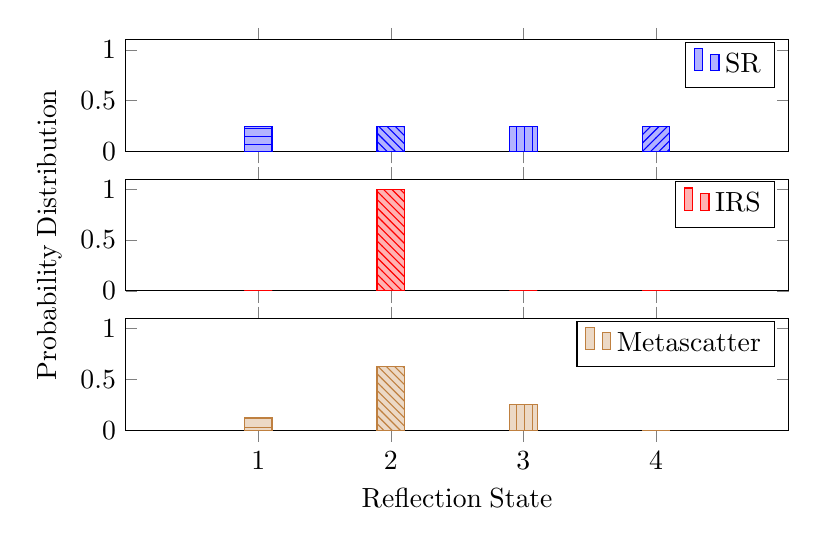
\begin{tikzpicture}
	\begin{groupplot}
		[group style={
					rows=3,
					group name=plots,
					x descriptions at=edge bottom,
					y descriptions at=edge left,
					vertical sep=10
				},
			ybar,
			xmin=0,
			xmax=4,
			xtick={1,2,3,4},
			ymin=0,
			ymax=1,
			xlabel={Reflection State},
			enlarge x limits={value=0.25,upper},
			enlarge y limits={value=0.1,upper},
			width=10cm,
			height=3cm,
			every axis plot/.append style={bar shift=0}
		]
		\nextgroupplot
		\addplot[blue,fill=blue!30!white] coordinates {(-1,-1)};
		\addplot[blue,fill=blue!30!white,postaction={pattern=horizontal lines},pattern color=.] coordinates {(1,0.25)};
		\addplot[blue,fill=blue!30!white,postaction={pattern=north west lines},pattern color=.] coordinates {(2,0.25)};
		\addplot[blue,fill=blue!30!white,postaction={pattern=vertical lines},pattern color=.] coordinates {(3,0.25)};
		\addplot[blue,fill=blue!30!white,postaction={pattern=north east lines},pattern color=.] coordinates {(4,0.25)};
		\legend{SR}
		\nextgroupplot[ylabel={Probability Distribution}]
		\addplot[red,fill=red!30!white] coordinates {(-1,-1)};
		\addplot[red,fill=red!30!white,postaction={pattern=horizontal lines},pattern color=.] coordinates {(1,0)};
		\addplot[red,fill=red!30!white,postaction={pattern=north west lines},pattern color=.] coordinates {(2,1)};
		\addplot[red,fill=red!30!white,postaction={pattern=vertical lines},pattern color=.] coordinates {(3,0)};
		\addplot[red,fill=red!30!white,postaction={pattern=north east lines},pattern color=.] coordinates {(4,0)};
		\legend{IRS}
		\nextgroupplot
		\addplot[brown,fill=brown!30!white] coordinates {(-1,-1)};
		\addplot[brown,fill=brown!30!white,postaction={pattern=horizontal lines},pattern color=.] coordinates {(1,0.125)};
		\addplot[brown,fill=brown!30!white,postaction={pattern=north west lines},pattern color=.] coordinates {(2,0.625)};
		\addplot[brown,fill=brown!30!white,postaction={pattern=vertical lines},pattern color=.] coordinates {(3,0.25)};
		\addplot[brown,fill=brown!30!white,postaction={pattern=north east lines},pattern color=.] coordinates {(4,0)};
		\legend{Metascatter}
	\end{groupplot}
\end{tikzpicture}

				}
				\label{fi:input_distribution}
			}
			\\
			\subfloat[Time Block]{
				\resizebox{0.8\columnwidth}{!}{
					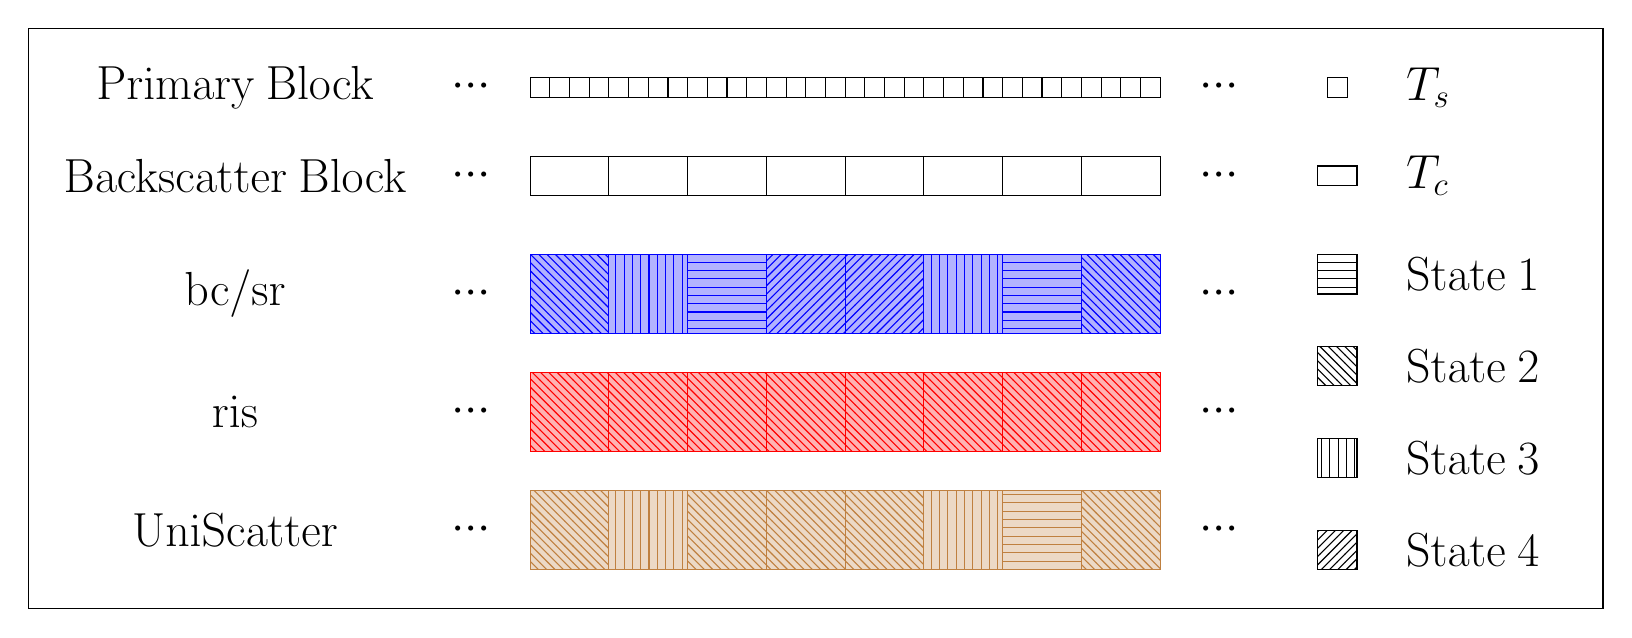
\begin{tikzpicture}
	\foreach \x in {0,...,31}{
			\draw (0.25*\x,3) rectangle ++(0.25,0.25);
		}
	\node[font=\LARGE] at (-0.75,3.125) {$\cdots$};
	\node[font=\LARGE] at (8.75,3.125) {$\cdots$};
	\node[font=\LARGE] at (-3.75,3.125) {Primary Block};
	\draw (10.125,3) rectangle ++(0.25,0.25);
	\node[font=\LARGE,right] at (11,3.125){$T_s$};

	\foreach \x in {0,...,7}{
			\draw (\x,1.75) rectangle ++(1,0.5);
		}
	\node[font=\LARGE] at (-0.75,2) {$\cdots$};
	\node[font=\LARGE] at (8.75,2) {$\cdots$};
	\node[font=\LARGE] at (-3.75,2) {Backscatter Block};
	\draw (10,1.875) rectangle ++(0.5,0.25);
	\node[font=\LARGE,right] at (11,2){$T_c$};

	\draw [blue,fill=blue!30!white,postaction={pattern=north west lines},pattern color=.](0,0) rectangle ++(1,1);
	\draw [blue,fill=blue!30!white,postaction={pattern=vertical lines},pattern color=.](1,0) rectangle ++(1,1);
	\draw [blue,fill=blue!30!white,postaction={pattern=horizontal lines},pattern color=.](2,0) rectangle ++(1,1);
	\draw [blue,fill=blue!30!white,postaction={pattern=north east lines},pattern color=.](3,0) rectangle ++(1,1);
	\draw [blue,fill=blue!30!white,postaction={pattern=north east lines},pattern color=.](4,0) rectangle ++(1,1);
	\draw [blue,fill=blue!30!white,postaction={pattern=vertical lines},pattern color=.](5,0) rectangle ++(1,1);
	\draw [blue,fill=blue!30!white,postaction={pattern=horizontal lines},pattern color=.](6,0) rectangle ++(1,1);
	\draw [blue,fill=blue!30!white,postaction={pattern=north west lines},pattern color=.](7,0) rectangle ++(1,1);
	\node[font=\LARGE] at (-0.75,0.5) {$\cdots$};
	\node[font=\LARGE] at (8.75,0.5) {$\cdots$};
	\node[font=\LARGE] at (-3.75,0.5) {\gls{bc}/\gls{sr}};

	\foreach \x in {0,...,7}{
			\draw [red,fill=red!30!white,postaction={pattern=north west lines},pattern color=.](\x,-1.5) rectangle ++(1,1);
		}
	\node[font=\LARGE] at (-0.75,-1) {$\cdots$};
	\node[font=\LARGE] at (8.75,-1) {$\cdots$};
	\node[font=\LARGE] at (-3.75,-1) {\gls{ris}};

	\draw [brown,fill=brown!30!white,postaction={pattern=north west lines},pattern color=.](0,-3) rectangle ++(1,1);
	\draw [brown,fill=brown!30!white,postaction={pattern=vertical lines},pattern color=.](1,-3) rectangle ++(1,1);
	\draw [brown,fill=brown!30!white,postaction={pattern=north west lines},pattern color=.](2,-3) rectangle ++(1,1);
	\draw [brown,fill=brown!30!white,postaction={pattern=north west lines},pattern color=.](3,-3) rectangle ++(1,1);
	\draw [brown,fill=brown!30!white,postaction={pattern=north west lines},pattern color=.](4,-3) rectangle ++(1,1);
	\draw [brown,fill=brown!30!white,postaction={pattern=vertical lines},pattern color=.](5,-3) rectangle ++(1,1);
	\draw [brown,fill=brown!30!white,postaction={pattern=horizontal lines},pattern color=.](6,-3) rectangle ++(1,1);
	\draw [brown,fill=brown!30!white,postaction={pattern=north west lines},pattern color=.](7,-3) rectangle ++(1,1);
	\node[font=\LARGE] at (-0.75,-2.5) {$\cdots$};
	\node[font=\LARGE] at (8.75,-2.5) {$\cdots$};
	\node[font=\LARGE] at (-3.75,-2.5) {UniScatter};

	\draw [pattern=horizontal lines](10,0.5) rectangle ++(0.5,0.5);
	\draw [pattern=north west lines](10,-2/3) rectangle ++(0.5,0.5);
	\draw [pattern=vertical lines](10,-11/6) rectangle ++(0.5,0.5);
	\draw [pattern=north east lines](10,-3) rectangle ++(0.5,0.5);
	\node[font=\LARGE,right] at (11,0.75){State 1};
	\node[font=\LARGE,right] at (11,-5/12){State 2};
	\node[font=\LARGE,right] at (11,-19/12){State 3};
	\node[font=\LARGE,right] at (11,-2.75){State 4};
	\draw (-6.375,-3.5) rectangle ++(20, 7.375);
\end{tikzpicture}

				}
				\label{fi:time_block}
			}
			\caption{
				Input probability distribution and time block structure of \gls{bc}, \gls{sr}, \gls{ris}, and UniScatter.
				$T_s$ and $T_c$ respectively denote the primary and backscatter symbol period.
				Within channel coherence time, UniScatter nodes semi-randomly select reflection state for each backscatter symbol block under the guidance of input probability distribution.
			}
			\label{fi:uniscatter_distribution}
		\end{figure}
		As illustrated in Fig. \ref{fi:uniscatter_distribution}, instead of always using fully random or deterministic reflection pattern over time, each UniScatter node can \emph{flexibly adjust} its input distribution to balance information encoding and channel reconfiguration.
		That is, it semi-randomly select the reflection state per backscatter symbol block under the guidance of input probability $P(\Gamma_m)$ for state $m$.
		Such an adaptive backscatter channel coding coincides with \gls{ris} when primary link is absolutely prioritized, and outperforms the uncoded equiprobable inputs of \gls{bc}/\gls{sr} when backscatter link is absolutely prioritized.
		Besides, the physically distributed characteristics of UniScatter nodes and legacy users avoids the development optimization and allows uniformly good performance for both links.

		As shown in Fig. \subref*{fi:block_diagram}, UniScatter nodes can be implemented over readily available passive backscatter devices with energy harvester and information decoder.
		Its equivalent circuit and scatter model are presented in Fig. \subref*{fi:equivalent_circuit} and \subref*{fi:scatter_model}.
		When activated by primary transmitter, each node harvests a proportion of the impinging wave for its own operation, decode the embedded coordination information for input distribution control, then applies a potentially random phase shift on the reradiated signal due to backscatter modulation.
		Energy harvesting and information decoding at passive UniScatter nodes can be realized using conventional power-splitting or time-sharing \gls{swipt} protocols \cite{Clerckx2019} or integrated energy-information receiver with pulse position modulated signal \cite{Kim2021a}.
		Besides, relevant \gls{csi} can be acquired using either traditional sequential methods \cite{Bharadia2015,Yang2015b,Guo2019g} or the state-of-the-art parallel approach \cite{Jin2021a}.
		In the following context, we assume perfect primary-backscatter coordination and perfect channel estimation for all links.
		\begin{figure*}[!t]
			\centering
			\subfloat[Block Diagram]{
				\resizebox{0.32\linewidth}{!}{
					% \begin{circuitikz}[transform shape]
% 	\tikzstyle{every node}=[font=\small]
% 	\coordinate (O) at (0,0);
% 	\node[block,from={O to $(O) + (6.375,3.25)$}](T){};
% 	\draw (0,1.75)
% 	to[short] ++(-0.875,0)
% 	to[short] ++(0,0.5) node[bareantenna](A){Bx};
% 	\draw (0,1.75)
% 	to[short,-*] ++(0.25,0) coordinate(J);
% 	\draw (J)
% 	to[short] ++(0,1)
% 	to[short] ++(0.5,0) coordinate(J1);
% 	\node[block,from={$(J1) + (0,-0.25)$ to $(J1) + (2.5,0.25)$}](R){Rectifier};
% 	\draw (J)
% 	to[short] ++(0.5,0) coordinate(J2);
% 	\node[block,from={$(J2) + (0,-0.25)$ to $(J2) + (2.5,0.25)$}](D){Demodulator};
% 	\draw (J)
% 	to[short] ++(0,-1)
% 	to[short] ++(0.5,0) coordinate(J3)
% 	to [vR,mirror,invert,/tikz/circuitikz/bipoles/length=1cm] ++(1.75,0) node[ground,rotate=90]{};
% 	\node[block,from={$(J3) + (0,-0.25)$ to $(J3) + (2.5,0.25)$},draw=none](M){};
% 	\draw ($(J3) + (0,-0.25)$) rectangle ($(J3) + (2.5,0.25)$);
% 	\draw ($(J3) + (1.25,-0.5)$) node[]{Modulator};
% 	\draw[dashed,-{Latex[length=2mm]}] (R.east) -- ++(0.75,0);
% 	\draw[-{Latex[length=2mm]}] (D.east) -- ++(0.75,0);
% 	\draw[{Latex[length=2mm]}-] (M.east) -- ++(0.75,0);
% 	\node[block,from={$(R.east) + (0.75,-0.25)$ to $(R.east) + (2.875,0.25)$}](P){Power Buffer};
% 	\node[block,from={$(M.east) + (0.75,-0.25)$ to $(D.east) + (2.875,0.25)$}](S){Digital\\Section};
% 	\draw[dashed,-{Latex[length=2mm]}] (P.south) to (S.north);
% 	\coordinate (F1) at ($(P.south)!0.5!(S.north)$);
% 	\coordinate (F2) at ($(D.east)!0.5!(S.west)$);
% 	\coordinate (F3) at ($(D.south)!0.5!(M.north)$);
% 	\draw[dashed] (F1) to (F1-|D.north);
% 	\draw[dashed,-{Latex[length=2mm]}] (F1-|D.north) to (D.north);
% 	\draw[dashed] (F1-|F2) to (F2|-F3) to (M|-F3);
% 	\draw[dashed,-{Latex[length=2mm]}] (M|-F3) to (M.north);
% \end{circuitikz}

\begin{circuitikz}[transform shape]
	\tikzstyle{every node}=[font=\small]
	\coordinate (O) at (0,0);
	\node[block,from={O to $(O) + (6.375,3)$}](T){};
	\draw (0,1.5)
	to[short] ++(-0.875,0)
	to[short] ++(0,0.5) node[bareantenna](A){Bx};
	\draw (0,1.5)
	to[short,-*] ++(0.25,0) coordinate(J);
	\draw (J)
	to[short] ++(0,1)
	to[short] ++(0.5,0) coordinate(J1);
	\node[block,from={$(J1) + (0,-0.25)$ to $(J1) + (2.5,0.25)$}](R){Rectifier};
	\draw (J)
	to[short] ++(0.5,0) coordinate(J2);
	\node[block,from={$(J2) + (0,-0.25)$ to $(J2) + (2.5,0.25)$}](D){Demodulator};
	\draw (J)
	to[short] ++(0,-1)
	to[short] ++(0.5,0) coordinate(J3);
	\node[block,from={$(J3) + (0,-0.25)$ to $(J3) + (2.5,0.25)$}](M){Modulator};
	\draw[dashed,-{Latex[length=2mm]}] (R.east) -- ++(0.75,0);
	\draw[-{Latex[length=2mm]}] (D.east) -- ++(0.75,0);
	\draw[{Latex[length=2mm]}-] (M.east) -- ++(0.75,0);
	\node[block,from={$(R.east) + (0.75,-0.25)$ to $(R.east) + (2.875,0.25)$}](P){Power Buffer};
	\node[block,from={$(M.east) + (0.75,-0.25)$ to $(D.east) + (2.875,0.25)$}](S){Digital\\Section};
	\draw[dashed,-{Latex[length=2mm]}] (P.south) to (S.north);
	\coordinate (F1) at ($(P.south)!0.5!(S.north)$);
	\coordinate (F2) at ($(D.east)!0.5!(S.west)$);
	\coordinate (F3) at ($(D.south)!0.5!(M.north)$);
	\draw[dashed] (F1) to (F1-|D.north);
	\draw[dashed,-{Latex[length=2mm]}] (F1-|D.north) to (D.north);
	\draw[dashed] (F1-|F2) to (F2|-F3) to (M|-F3);
	\draw[dashed,-{Latex[length=2mm]}] (M|-F3) to (M.north);
\end{circuitikz}

				}
				\label{fi:block_diagram}
			}
			\subfloat[Equivalent Circuit]{
				\resizebox{0.37\linewidth}{!}{
					\begin{circuitikz}[transform shape]
	\tikzstyle{every node}=[font=\Large]
	\draw (0,0) coordinate(O)
	to [sV,l=$V_0$] ++(0,1.5)
	to [L,l=$X_{\text{A}}$] ++(0,1.5)
	to [R=$R_{\text{A}}$,-*] ++(3,0) coordinate(AM)
	to [sI,l_=$I_0$,-*] ++(0,-3)
	to [short] (O);
	\draw (AM)
	to [short] ++(0.5,0)
	to [L,l=$X_m$,-*] ++(3,0) coordinate(M)
	to [R=$R_{\text{S},m}$] ++(3,0) coordinate(MH);
	\draw (M)
	to [R=$R_{\text{P},m}$,-*] ++(0,-3);
	\draw (MH)
	to [D,-*] ++(1.5,0) coordinate(H)
	to [C=$X_{\text{H}}$,-*] ++(0,-3);
	\draw (H)
	to [short] ++(1.5,0)
	to [R=$R_{\text{H}}$] ++(0,-3)
	to [short] (O);

	\draw [dashed] (-1.125,-0.5) rectangle (3.5,4);
	\draw [dashed] (4,-0.5) rectangle (9,4);
	\draw [dashed] (9.5,-0.5) rectangle (13.5,4);

	\draw (1.125,4.25) node[]{Antenna};
	\draw (6.5,4.25) node[]{Modulator};
	\draw (11.5,4.25) node[]{Harvester \& Chip};

	\draw (3.375,2.675) to [short] (3.375,3.175) to [short] (3.25,3.175) to [short,i_=$Z_{\text{A}}$] (3.125,3.175);
	\draw (4.125,-0.125) to [short] (4.125,0.375) to [short] (4.25,0.375) to [short,i=$Z_m$] (4.375,0.375);
	\draw (9.625,-0.125) to [short] (9.625,0.375) to [short] (9.75,0.375) to [short,i=$Z_{\text{H}}$] (9.875,0.375);
\end{circuitikz}

				}
				\label{fi:equivalent_circuit}
			}
			\subfloat[Scatter Model]{
				\resizebox{0.28\linewidth}{!}{
					\begin{circuitikz}[transform shape]
	\tikzstyle{every node}=[font=\large]
	\ctikzset{multipoles/rotary/arrow=both}
	\draw (0,0) node[bareantenna](bareantenna){};
	\draw (bareantenna.west) ++(-1,0) node[waves](WI){};
	\draw (WI.north east) ++(0.25,0) node{$\vec{E}_{\mathrm{I}}$};
	\draw (WI.south east) ++(0.25,0) node{$\vec{H}_{\mathrm{I}}$};
	\draw (bareantenna.east) ++(0.5,0) node[waves](WR){};
	\draw (WR.north east) ++(0.35,0) node{$\vec{E}_m$};
	\draw (WR.south east) ++(0.35,0) node{$\vec{H}_m$};
	\draw (bareantenna) to ++(0,-1.1) to [generic,l=$Z_{\mathrm{A}}$,/tikz/circuitikz/bipoles/length=0.75cm] ++(2.3,0) node[rotary switch=4 in 90 wiper 30,anchor=ext center,rotate=0](SW){};
	\draw (SW.cout 1) to ++(0.625,+0.5) to [generic,/tikz/circuitikz/bipoles/length=0.75cm] ++(2.2,0) coordinate(E1);
	\draw (SW.cout 2) node[above right]{$m$} to [generic,l=$Z_m$,/tikz/circuitikz/bipoles/length=0.75cm] ++(2.2,0) coordinate(E2);
	\draw (SW.cout 3) to [generic,/tikz/circuitikz/bipoles/length=0.75cm] ++(2.2,0) coordinate(E3);
	\draw (SW.cout 4) to ++(0.625,-0.5) to [generic,/tikz/circuitikz/bipoles/length=0.75cm] ++(2.2,0) coordinate(E4);
	\draw (E1) to[short,-*] (E2);
	\draw (E2) to[short,-*] (E3);
	\draw (E3) to[short] (E4);
	\draw (E2) to[short] ++(0.2,0) node[ground,rotate=90]{};
\end{circuitikz}

				}
				\label{fi:scatter_model}
			}
			\caption{Block diagram, equivalent circuit, and scatter model of a UniScatter node. The solid and dashed vectors represent signal and energy flows. The scattering antenna behaves as a constant power source, where the voltage $V_0$ and current $I_0$ are introduced by incident electric field $\vec{E}_{\mathrm{I}}$ and magnetic field $\vec{H}_{\mathrm{I}}$ \cite{Huang2021}.}
			\label{fi:uniscatter_node}
		\end{figure*}
	\end{subsection}

	\begin{subsection}{UniScatter Receiver}
		Since each passive UniScatter node directly modulates its own message over the legacy signal, it involves a \emph{double modulation} where the primary and backscatter symbols are superimposed by \emph{multiplication coding} instead of superposition coding.
		Besides, the backscatter symbol period is typically longer than primary due to the load switching speed constraint.
		Those facts imply \emph{backscatter detection} under primary uncertainty can be viewed as part of \emph{primary channel training}.
		Hence, we propose a practical UniScatter receiver that semi-coherently decodes UniScatter nodes from the received energy per backscatter block, re-encodes for their reflection patterns, retrieves equivalent primary channel as if dynamic passive beamforming, then coherently decodes the primary link under the enhanced multipath.
		\begin{figure}[!t]
			\centering
			\resizebox{0.9\columnwidth}{!}{
				\definecolor{color1}{HTML}{0072BD}
\definecolor{color2}{HTML}{D95319}
\definecolor{color3}{HTML}{EDB120}
\definecolor{color4}{HTML}{7E2F8E}

\begin{tikzpicture}
	\begin{axis}[
			clip mode=individual,
			height=5cm,
			width=9cm,
			xlabel = $z$,
			ylabel = {Probability Density},
			font=\scriptsize,
			no markers,
			xmin=0,
			ymin=0,
			xmax=70,
			xtick={0,12.78,20.28,29.62,70},
			xticklabels={$t_0$,$t_1$,$t_2$,$t_3$,$t_4$},
			yticklabels=\empty,
			samples = 200
		]

		\addplot+[very thick,solid,color1] gnuplot[raw gnuplot] {%
				isint(x) = (int(x)==x);
				gmm(x,rho,lambda)=rho<=0||lambda<=0?1/0:  x<0?0.0:x==0?(rho>1?0.0:rho==1?real(lambda):1/0):  exp(rho*log(lambda)+(rho-1.0)*log(x)-lgamma(rho)-lambda*x);
				set xrange [0:80];
				set yrange [0:1];
				samples=200;
				plot gmm(x,10,1)};
		\addlegendentryexpanded{$f(z \mid \mathcal{H}_1)$}

		\addplot+[very thick,dashed,color2] gnuplot[raw gnuplot] {%
				isint(x) = (int(x)==x);
				gmm(x,rho,lambda)=rho<=0||lambda<=0?1/0:  x<0?0.0:x==0?(rho>1?0.0:rho==1?real(lambda):1/0):  exp(rho*log(lambda)+(rho-1.0)*log(x)-lgamma(rho)-lambda*x);
				set xrange [0:80];
				set yrange [0:1];
				samples=200;
				plot gmm(x,10,0.6)};
		\addlegendentryexpanded{$f(z \mid \mathcal{H}_2)$}

		\addplot+[very thick,dotted,color3] gnuplot[raw gnuplot] {%
				isint(x) = (int(x)==x);
				gmm(x,rho,lambda)=rho<=0||lambda<=0?1/0:  x<0?0.0:x==0?(rho>1?0.0:rho==1?real(lambda):1/0):  exp(rho*log(lambda)+(rho-1.0)*log(x)-lgamma(rho)-lambda*x);
				set xrange [0:80];
				set yrange [0:1];
				samples=200;
				plot gmm(x,10,0.4)};
		\addlegendentryexpanded{$f(z \mid \mathcal{H}_3)$}

		\addplot+[very thick,dashdotted,color4] gnuplot[raw gnuplot] {%
				isint(x) = (int(x)==x);
				gmm(x,rho,lambda)=rho<=0||lambda<=0?1/0:  x<0?0.0:x==0?(rho>1?0.0:rho==1?real(lambda):1/0):  exp(rho*log(lambda)+(rho-1.0)*log(x)-lgamma(rho)-lambda*x);
				set xrange [0:80];
				set yrange [0:1];
				samples=200;
				plot gmm(x,10,0.28)};
		\addlegendentryexpanded{$f(z \mid \mathcal{H}_4)$}
		\draw[latex-latex] (0,0) -- (12.78,0) node[above,midway,yshift=-2]{$\mathcal{R}_1$};
		\draw[latex-latex] (12.78,0) -- (20.28,0) node[above,midway,yshift=-2]{$\mathcal{R}_2$};
		\draw[latex-latex] (20.28,0) -- (29.62,0) node[above,midway,yshift=-2]{$\mathcal{R}_3$};
		\draw[latex-latex] (29.62,0) -- (70,0) node[above,midway,yshift=-2]{$\mathcal{R}_4$};
	\end{axis}
\end{tikzpicture}

			}
			\caption{
				\gls{pdf} of total received energy per backscatter block, conditioned on different input state hypotheses.
				$t$ and $\mathcal{R}$ denote the energy decision thresholds and regions, respectively.
			}
			\label{fi:energy_distribution}
		\end{figure}
		As illustrated in Fig. \ref{fi:energy_distribution}, the total received energy per backscatter block is a random variable that follows different distributions conditioned on different input state hypotheses.
		Compared with conventional joint \gls{ml} and \gls{sic} from stronger primary link to weaker backscatter links, UniScatter receiver not only preserves the benefits of backscatter modulation and passive beamforming, but also enjoys much lower computational and operational complexities.
	\end{subsection}

	\begin{subsection}{System Model}
		\begin{figure}[!t]
			\centering
			\def\svgwidth{0.8\columnwidth}
			\footnotesize{
				\import{assets/illustration/}{uniscatter_network.eps_tex}
			}
			\caption{A single-user multi-node UniScatter network.}
			\label{fi:uniscatter_network}
		\end{figure}
		To demonstrate the advantages of UniScatter, we consider a single-user multi-node \gls{miso} UniScatter network as shown in Fig. \ref{fi:uniscatter_network}.
		In the primary active point-to-point system, a $Q$-antenna \gls{ap} transmits to a single-antenna user assisted by $K$ nearby single-antenna UniScatter nodes with $M$ reflection states.
		In the secondary backscatter \gls{mac} system, the \gls{ap} serves as the carrier emitter, the distributed UniScatter nodes modulate information over reradiated \gls{rf} signals, and the user decodes their messages.
		For simplicity, we consider a quasi-static block fading model where channels remain constant within coherence block and vary independently between consecutive blocks.
		Due to the physical constraints of load switching speed, we assume the backscatter over primary symbol period ratio is an integer $N \gg 1$.
		We also omit the signal reflected by two or more times and ignore the propagation time difference of different paths.

		Denote the \gls{ap}-user direct channel as $\boldsymbol{h}_{\mathrm{D}}^H \in \mathbb{C}^{1 \times Q}$, the \gls{ap}-node $k \in \mathcal{K} \triangleq \{1,\ldots,K\}$ forward channel as $\boldsymbol{h}_{\mathrm{F},k}^H \in \mathbb{C}^{1 \times Q}$, the node $k$-user backward channel as $h_{\mathrm{B},k}$, and the cascaded channel via tag $k$ as $\boldsymbol{h}_{\mathrm{C},k}^H \triangleq h_{\mathrm{B},k} \boldsymbol{h}_{\mathrm{F},k}^H \in \mathbb{C}^{1 \times Q}$.
		Let $x_{\mathcal{K}} \triangleq (x_1,\ldots,x_K)$ be the backscatter symbol tuple of all UniScatter nodes.
		Without loss of generality, we consider one specific backscatter block (i.e., $N$ primary blocks) in the following context.
		Due to double modulation, the equivalent primary channel is a function of \emph{coded} backscatter symbols
		% \begin{subequations}
		% 	\label{eq:equivalent_channel}
		% 	\begin{align}
		% 		\boldsymbol{h}_{\mathrm{E}}^H(x_{\mathcal{K}})
		% 		 & \triangleq \boldsymbol{h}_{\mathrm{D}}^H + \sum_{k \in \mathcal{K}} \alpha_k \boldsymbol{h}_{\mathrm{C},k}^H x_k   \\
		% 		 & = \boldsymbol{h}_{\mathrm{D}}^H + \boldsymbol{x}^H \mathrm{diag}(\boldsymbol{\alpha}) \boldsymbol{H}_{\mathrm{C}},
		% 	\end{align}
		% \end{subequations}
		\begin{equation}
			\boldsymbol{h}_{\mathrm{E}}^H(x_{\mathcal{K}}) \triangleq \boldsymbol{h}_{\mathrm{D}}^H + \sum_{k \in \mathcal{K}} \alpha_k \boldsymbol{h}_{\mathrm{C},k}^H x_k = \boldsymbol{h}_{\mathrm{D}}^H + \boldsymbol{x}^H \mathrm{diag}(\boldsymbol{\alpha}) \boldsymbol{H}_{\mathrm{C}},
			\label{eq:equivalent_channel}
		\end{equation}
		where $\alpha_k \in \mathbb{I}$ is the amplitude scattering ratio of UniScatter node $k$, $x_k \in \mathcal{X} \triangleq \{c_1,\ldots,c_M\}$ is the \emph{coded} backscatter symbol of node $k$, $\boldsymbol{\alpha} \triangleq [\alpha_1,\ldots,\alpha_K]^T \in \mathbb{I}^{K \times 1}$, $\boldsymbol{x} \triangleq [x_1,\ldots,x_K]^H \in \mathcal{X}^{K \times 1}$, and $\boldsymbol{H}_{\mathrm{C}} \triangleq [\boldsymbol{h}_{\mathrm{C},1},\ldots,\boldsymbol{h}_{\mathrm{C},K}]^H \in \mathbb{C}^{K \times Q}$. The signal received by the user at primary block $n \in \mathcal{N} \triangleq \{1,\ldots,N\}$ is
		\begin{equation}
			y[n] = \boldsymbol{h}_{\mathrm{E}}^H(x_{\mathcal{K}}) \boldsymbol{w} s[n] + v[n],
			\label{eq:receive_signal}
		\end{equation}
		where $s \sim \mathcal{CN}(0,1)$ is the primary symbol, $v \sim \mathcal{CN}(0,\sigma_v^2)$ is the \gls{awgn}, and $\boldsymbol{w} \in \mathbb{C}^{Q \times 1}$ is the active beamforming vector subject to average transmit power constraint $\lVert \boldsymbol{w} \rVert^2 \le P$.
		Denote $m_k \in \mathcal{M} \triangleq \{1,\ldots,M\}$ as the reflection state index of node $k$, and $m_{\mathcal{K}} \triangleq (m_1,\ldots,m_K)$ as the state index tuple of all nodes.
		Conditioned on backscatter index tuple $m_{\mathcal{K}}$, the received signal \eqref{eq:receive_signal} follows \gls{cscg} distribution $y[n] \sim \mathcal{CN}(0,\sigma_{m_{\mathcal{K}}}^2)$, where
		\begin{equation}
			\sigma_{m_{\mathcal{K}}}^2 = \lvert \boldsymbol{h}_{\mathrm{E}}^H(x_{m_{\mathcal{K}}}) \boldsymbol{w} \rvert^2 + \sigma_v^2
			\label{eq:receive_variance}
		\end{equation}
		is the received variance and $x_{m_\mathcal{K}}$ is the backscatter symbol tuple associated with $m_{\mathcal{K}}$.
		For node $k$, let $x_{m_k}$ be the backscatter symbol associated with index $m_k$.%
		\footnote{
			Please note $x_k$ and $x_{\mathcal{K}}$ are random variable and tuple, while $x_{m_k}$ and $x_{m_{\mathcal{K}}}$ are their instances of index $m_k$ and $m_{\mathcal{K}}$.
		}
		Besides, we define the total received energy per backscatter block as $z=\sum_{n=1}^N \lvert y[n] \rvert^2$.
		Since $z$ is the sum of $N$ \gls{iid} exponential variables, its \gls{pdf} conditioned on $m_{\mathcal{K}}$ follows Gamma distribution
		\begin{equation}
			f(z|\mathcal{H}_{m_{\mathcal{K}}}) = \frac{z^{N-1} \exp(-z/\sigma_{m_{\mathcal{K}}}^2)}{\sigma_{m_{\mathcal{K}}}^{2N} (N-1)!},
			\label{eq:energy_distribution}
		\end{equation}
		where $\mathcal{H}_{m_{\mathcal{K}}}$ denotes hypothesis $m_{\mathcal{K}}$.
		As illustrated in Fig. \ref{fi:energy_distribution}, the UniScatter receiver divides the received energy space into disjoint decision regions associated with those hypotheses.
		For example, if the total received energy during a backscatter block falls within region $\mathcal{R}_{m_{\mathcal{K}}}$, then the detector output would be $x_{m_{\mathcal{K}}}$.
		\begin{remark}
			Interestingly, the capacity-achieving decision design for \gls{dmtc} remains under-investigated, and some attempts were made for a single source with binary inputs \cite{Qian2019b,Nguyen2021b}.
			For non-binary inputs with arbitrary distribution, the optimal decision region for each letter can be non-convex (i.e., with non-adjacent partitions) and the optimal number of thresholds is still unknown \cite{Nguyen2018,Nguyen2021}.
		\end{remark}
		Like most existing literatures, we limit the scope of this paper to convex decision regions and consider sequential decision thresholds design therein.
		For the ease of notations, we define a general bijective function transforming backscatter index tuple $m_{\mathcal{K}}$ to integer $l \in \mathcal{L} \triangleq \{1,\ldots,L \triangleq M^K\}$, and use both notation interchangeably in the following context.
		As such, the convex decision region of backscatter index tuple $m_{\mathcal{K}}$ or equivalent letter $l$ can be written as
		\begin{equation}
			\mathcal{R}_{m_{\mathcal{K}}} \triangleq [t_{l-1},t_l), \quad t_{l-1} \le t_l.
		\end{equation}
		Once the decision threshold vector $\boldsymbol{t} \triangleq [t_0,\ldots,t_L]^T \in \mathbb{R}_+^{(L+1) \times 1}$ is determined, we can formulate a \gls{dmtmac} with transition probability from input $x_{m_{\mathcal{K}}}$ to output $\hat{x}_{m_{\mathcal{K}}'}$
		\begin{equation}
			P(\hat{x}_{m_{\mathcal{K}}'}|x_{m_{\mathcal{K}}}) = \int_{\mathcal{R}_{m_{\mathcal{K}}'}} f(z|\mathcal{H}_{m_{\mathcal{K}}}) \, d z,
			\label{eq:dmtmac}
		\end{equation}
		then perform backscatter channel coding on top of it.
	\end{subsection}

	\begin{subsection}{Information Theory}
		Denote the input probability distribution vector of node $k$ as $\boldsymbol{p}_k \triangleq [P_k(c_1),\ldots,P_k(c_M)]^T \in \mathbb{I}^{M \times 1}$, and the probability of state $m_k$ as $P_k(x_{m_k})$.
		With independent encoding at all nodes, the probability of backscatter symbol tuple $x_{m_{\mathcal{K}}}$ is
		\begin{equation}
			P_{\mathcal{K}}(x_{m_{\mathcal{K}}}) = \prod_{k \in \mathcal{K}} P_k(x_{m_k}).
			\label{eq:equivalent_distribution}
		\end{equation}

		Similar to \cite{Rezaeian2004}, we define the backscatter information function between input symbol tuple instance $x_{m_{\mathcal{K}}}$ and output symbol tuple variable $\hat{x}_{\mathcal{K}}$ as
		\begin{equation}
			I_{\mathrm{B}}(x_{m_{\mathcal{K}}};\hat{x}_{\mathcal{K}}) \triangleq \sum_{m_{\mathcal{K}}'} P(\hat{x}_{m_{\mathcal{K}}'}|x_{m_{\mathcal{K}}}) \log \frac{P(\hat{x}_{m_{\mathcal{K}}'}|x_{m_{\mathcal{K}}})}{P_{\mathcal{K}}(\hat{x}_{m_{\mathcal{K}}'})},
			\label{eq:backscatter_information_function}
		\end{equation}
		where $P_{\mathcal{K}}(\hat{x}_{m_{\mathcal{K}}'}) = \sum_{m_{\mathcal{K}}} P_{\mathcal{K}}(x_{m_{\mathcal{K}}}) P(\hat{x}_{m_{\mathcal{K}}'}|x_{m_{\mathcal{K}}})$ is the probability of channel output tuple $\hat{x}_{m_{\mathcal{K}}'}$.
		We also define the backscatter marginal information of letter $x_{m_k}$ of node $k$ as
		\begin{equation}
			I_{\mathrm{B},k}(x_{m_k};\hat{x}_{\mathcal{K}}) \triangleq \sum_{m_{\mathcal{K} \setminus \{k\}}} P_{\mathcal{K} \setminus \{k\}}(x_{m_{\mathcal{K} \setminus \{k\}}}) I_{\mathrm{B}}(x_{m_{\mathcal{K}}};\hat{x}_{\mathcal{K}}),
			\label{eq:backscatter_marginal_information}
		\end{equation}
		where $P_{\mathcal{K} \setminus \{k\}}(x_{m_{\mathcal{K} \setminus \{k\}}}) = \prod_{q \in \mathcal{K} \setminus \{k\}} P_{q}(x_{m_{q}})$.
		The backscatter mutual information can be written as
		\begin{equation}
			I_{\mathrm{B}}(x_{\mathcal{K}};\hat{x}_{\mathcal{K}}) = \sum_{m_{\mathcal{K}}} P_{\mathcal{K}}(x_{m_{\mathcal{K}}}) I_{\mathrm{B}}(x_{m_{\mathcal{K}}};\hat{x}_{\mathcal{K}}).
			\label{eq:backscatter_mutual_information}
		\end{equation}
		Once backscatter messages of all nodes are successfully decoded, we can re-code for backscatter symbol tuple $x_{\mathcal{K}}$, recover their reflection patterns by \eqref{eq:backscatter_modulation}, and retrieve the equivalent primary channel by \eqref{eq:equivalent_channel}.
		Moreover, we define the primary information function conditioned on backscatter symbol tuple $x_{m_{\mathcal{K}}}$ as
		\begin{equation}
			I_{\mathrm{P}}(s;y|x_{m_{\mathcal{K}}}) \triangleq \log \Bigl(1 + \frac{\lvert \boldsymbol{h}_{\mathrm{E}}^H(x_{m_{\mathcal{K}}}) \boldsymbol{w} \rvert^2}{\sigma_v^2}\Bigr),
			\label{eq:primary_information_function}
		\end{equation}
		the primary marginal information conditioned on letter $x_{m_k}$ of node $k$ as
		\begin{equation}
			I_{\mathrm{P},k}(s;y|x_{m_k}) \triangleq \sum_{m_{\mathcal{K} \setminus \{k\}}} P_{\mathcal{K} \setminus \{k\}}(x_{m_{\mathcal{K} \setminus \{k\}}}) I_{\mathrm{P}}(s;y|x_{m_{\mathcal{K}}}),
			\label{eq:primary_marginal_information}
		\end{equation}
		and the primary ergodic mutual information as
		\begin{equation}
			I_{\mathrm{P}}(s;y|x_{\mathcal{K}}) = \sum_{m_{\mathcal{K}}} P_{\mathcal{K}}(x_{m_{\mathcal{K}}}) I_{\mathrm{P}}(s;y|x_{m_{\mathcal{K}}}).
			\label{eq:primary_mutual_information}
		\end{equation}

		With a slight abuse of notation, we define the corresponding weighted sum information function, marginal information, and mutual information respectively as
		\begin{align}
			I(x_{m_{\mathcal{K}}})
			 & \triangleq \rho I_{\mathrm{P}}(s;y|x_{m_{\mathcal{K}}}) + (1 - \rho) I_{\mathrm{B}}(x_{m_{\mathcal{K}}};\hat{x}_{\mathcal{K}}),\label{eq:weighted_sum_information_function} \\
			I_k(x_{m_k})
			 & \triangleq \rho I_{\mathrm{P},k}(s;y|x_{m_k}) + (1 - \rho) I_{\mathrm{B},k}(x_{m_k};\hat{x}_{\mathcal{K}}),\label{eq:weighted_sum_marginal_information}                     \\
			I(x_{\mathcal{K}})
			 & \triangleq \rho I_{\mathrm{P}}(s;y|x_{\mathcal{K}}) + (1 - \rho) I_{\mathrm{B}}(x_{\mathcal{K}};\hat{x}_{\mathcal{K}}),\label{eq:weighted_sum_mutual_information}
		\end{align}
		where $\rho \in \mathbb{I}$ is the relative priority of the primary link.
	\end{subsection}
	\label{se:uniscatter}
\end{section}

\begin{section}{Rate-Region Characterization}
	To characterize the achievable primary-total-backscatter rate region of the proposed UniScatter system, we aim to maximize the weighted sum mutual information with respect to input distribution $\{\boldsymbol{p}_k\}_{k \in \mathcal{K}}$, active beamforming $\boldsymbol{w}$, and decision thresholds $\boldsymbol{t}$ as
	\begin{maxi!}
		{\scriptstyle{\{\boldsymbol{p}_k\}_{k \in \mathcal{K}},\boldsymbol{w},\boldsymbol{t}}}{I(x_{\mathcal{K}})}{\label{op:weighted_sum_rate}}{\label{ob:weighted_sum_rate}}
		\addConstraint{\boldsymbol{1}^T \boldsymbol{p}_k}{=1,}{\quad \forall k}{\label{co:sum_probability}}
		\addConstraint{\boldsymbol{p}_k}{\ge \boldsymbol{0},}{\quad \forall k}{\label{co:nonnegative_probability}}
		\addConstraint{\lVert \boldsymbol{w} \rVert^2}{\le P}{\label{co:transmit_power}}
		\addConstraint{t_{l-1}}{\le t_l,}{\quad \forall l.}{\label{co:decision_threshold}}
	\end{maxi!}
	Since problem \eqref{op:weighted_sum_rate} is highly non-convex, we propose a \gls{bcd} algorithm that iteratively updates $\{\boldsymbol{p}_k\}_{k \in \mathcal{K}}$, $\boldsymbol{w}$ and $\boldsymbol{t}$ until convergence.

	\begin{subsection}{Input Distribution}
		For any given $\boldsymbol{w}$ and $\boldsymbol{t}$, we can construct the equivalent \gls{dmtmac} by \eqref{eq:dmtmac} and simplify \eqref{op:weighted_sum_rate} to
		\begin{maxi!}
			{\scriptstyle{\{\boldsymbol{p}_k\}_{k \in \mathcal{K}}}}{I(x_{\mathcal{K}})}{\label{op:input_distribution}}{}
			\addConstraint{\eqref{co:sum_probability},\eqref{co:nonnegative_probability},}
		\end{maxi!}
		which involves the coupled term $\prod_{k \in \mathcal{K}} P_k(x_{m_k})$ and is non-convex when $K > 1$.
		Following \cite{Rezaeian2004}, we first recast \gls{kkt} conditions of problem \eqref{op:input_distribution} to their equivalent forms, then propose a numerical method that guarantees those conditions on convergence of sequences.
		% ? Next, we propose a numerical method that evaluate the \gls{kkt} input distribution by limit of sequences.
		\begin{remark}
			As demonstrated in \cite{Buhler2011}, \gls{kkt} conditions are generally necessary but insufficient for total rate maximization problems.
			Although \gls{kkt} solutions to problem \eqref{op:input_distribution} may end up being saddle points, we will later show by simulation their average performance can be reasonably close to optimal for a moderate $K$.
		\end{remark}
		\begin{proposition}
			The \gls{kkt} optimality conditions for problem \eqref{op:input_distribution} are equivalent to, $\forall k,m_k$,
			\begin{subequations}
				\label{eq:input_kkt_condition}
				\begin{alignat}{2}
					I_k^\star(x_{m_k}) & = I^\star(x_{\mathcal{K}}), \quad   &  & P_k^\star(x_{m_k}) > 0,\label{eq:probable_states} \\
					I_k^\star(x_{m_k}) & \le I^\star(x_{\mathcal{K}}), \quad &  & P_k^\star(x_{m_k}) = 0.\label{eq:dropped_states}
				\end{alignat}
			\end{subequations}
			\label{pr:input_kkt_condition}
		\end{proposition}

		\begin{proof}
			Please refer to Appendix \ref{ap:input_kkt_condition}.
			\label{pf:input_kkt_condition}
		\end{proof}

		For each node, \eqref{eq:probable_states} suggests each probable state should produce the same marginal information (averaged over all states of other nodes), while \eqref{eq:dropped_states} suggests any state with potentially less marginal information should not be used.
		\begin{proposition}
			For any strictly positive initializer $\{\boldsymbol{p}_k^{(0)}\}_{k \in \mathcal{K}}$, the \gls{kkt} input probability of node $k$ at state $m_k$ is given by the converging point of the sequence
			\begin{equation}
				P_k^{(r+1)}(x_{m_k}) = \frac{P_k^{(r)}(x_{m_k}) \exp \Bigl( \frac{\rho}{1 - \rho} I_k^{(r)}(x_{m_k}) \Bigr)}{\sum_{m_k'} P_k^{(r)}(x_{m_k'}) \exp \Bigl( \frac{\rho}{1 - \rho} I_k^{(r)}(x_{m_k'}) \Bigr)},
				\label{eq:input_kkt_solution}
			\end{equation}
			where $r$ is the iteration index.
			\label{pr:input_kkt_solution}
		\end{proposition}
		\begin{proof}
			Please refer to Appendix \ref{ap:input_kkt_solution}.
			\label{pf:input_kkt_solution}
		\end{proof}

		For \eqref{eq:input_kkt_solution} at iteration $r+1$, the input distribution of node $k$ is updated over $\bigl\{\{\boldsymbol{p}_q^{(r+1)}\}_{q=1}^{k-1},\{\boldsymbol{p}_q^{(r)}\}_{q=k}^{K}\bigr\}$.
		The \gls{kkt} input distribution design is summarized in Algorithm \ref{al:input_distribution}.

		\begin{algorithm}[!t]
			\caption{Numerical \gls{kkt} Input Distribution Evaluation by Limits of Sequence}
			\label{al:input_distribution}
			\begin{algorithmic}[1]
				\Require $K$, $N$, $\boldsymbol{h}_{\mathrm{D}}^H$, $\boldsymbol{H}_{\mathrm{C}}$, $\boldsymbol{\alpha}$, $\mathcal{X}$, $\sigma_v^2$, $\rho$, $\boldsymbol{w}$, $\boldsymbol{t}$, $\epsilon$
				\Ensure $\{\boldsymbol{p}_k^\star\}_{k \in \mathcal{K}}$
				\State Set $\boldsymbol{h}_{\mathrm{E}}^H(x_{m_{\mathcal{K}}})$, $\forall m_{\mathcal{K}}$ by \eqref{eq:equivalent_channel}
				\State \phantom{Set} $\sigma^2_{m_{\mathcal{K}}}$, $\forall m_{\mathcal{K}}$ by \eqref{eq:receive_variance}
				\State \phantom{Set} $f(z|\mathcal{H}_{m_{\mathcal{K}}})$, $\forall m_{\mathcal{K}}$ by \eqref{eq:energy_distribution}
				\State \phantom{Set} $P(\hat{x}_{m_{\mathcal{K}}'}|x_{m_{\mathcal{K}}})$, $\forall m_{\mathcal{K}}, m_{\mathcal{K}}'$ by \eqref{eq:dmtmac}
				\State Initialize $r \gets 0$
				\State \phantom{Initialize} $\boldsymbol{p}_k^{(0)} > \boldsymbol{0}$, $\forall k$
				\State Get $P_{\mathcal{K}}^{(r)}(x_{m_{\mathcal{K}}})$, $\forall m_{\mathcal{K}}$ by \eqref{eq:equivalent_distribution} \label{st:input_distribution_begin}
				\State \phantom{Get} $I^{(r)}(x_{m_{\mathcal{K}}})$, $\forall m_{\mathcal{K}}$ by \eqref{eq:backscatter_information_function}, \eqref{eq:primary_information_function}, \eqref{eq:weighted_sum_information_function}
				\State \phantom{Get} $I^{(r)}_k(x_{m_k})$, $\forall k,m_k$ by \eqref{eq:backscatter_marginal_information}, \eqref{eq:primary_marginal_information}, \eqref{eq:weighted_sum_marginal_information}
				\State \phantom{Get} $I^{(r)}(x_{\mathcal{K}})$ by \eqref{eq:backscatter_mutual_information}, \eqref{eq:primary_mutual_information}, \eqref{eq:weighted_sum_mutual_information} \label{st:input_distribution_end}
				\Repeat
					\State Update $r \gets r+1$
					\State \phantom{Update} $\boldsymbol{p}_k^{(r)}$, $\forall k$ by \eqref{eq:input_kkt_solution}
					\State Redo step \ref{st:input_distribution_begin}--\ref{st:input_distribution_end}
				\Until $I^{(r)}(x_{\mathcal{K}}) - I^{(r-1)}(x_{\mathcal{K}}) \le \epsilon$
			\end{algorithmic}
		\end{algorithm}
	\end{subsection}

	\begin{subsection}{Active Beamforming}
		For any given $\{\boldsymbol{p}_k\}_{k \in \mathcal{K}}$ and $\boldsymbol{t}$, problem \eqref{op:weighted_sum_rate} reduces to
		\begin{maxi!}
			{\scriptstyle{\boldsymbol{w}}}{I(x_{\mathcal{K}})}{\label{op:active_beamforming}}{\label{ob:active_beamforming}}
			\addConstraint{\eqref{co:transmit_power},}
		\end{maxi!}
		which is still non-convex due to the integration and entropy terms.
		To tackle this, we rewrite the \gls{dmtmac} transition probability \eqref{eq:dmtmac} from input index tuple $m_{\mathcal{K}}$ to output index $l$ as a regularized incomplete Gamma function in the series representation \cite[Theorem~3]{Jameson2016}
		\begin{equation}
			\begin{gathered}
				Q\Bigl(N,\frac{t_{l-1}}{\sigma_{m_{\mathcal{K}}}^2},\frac{t_l}{\sigma_{m_{\mathcal{K}}}^2}\Bigr) = \frac{\int_{{t_{l-1}}/{\sigma_{m_{\mathcal{K}}}^2}}^{{t_l}/{\sigma_{m_{\mathcal{K}}}^2}} z^{N-1} \exp(-z) \, d z}{(N-1)!}\\
				= \exp \Bigl(-\frac{t_{l-1}}{\sigma_{m_{\mathcal{K}}}^2}\Bigr) \sum_{n=0}^{N-1} \frac{\bigl(\frac{t_{l-1}}{\sigma_{m_{\mathcal{K}}}^2}\bigr)^n}{n!} - \exp \Bigl(-\frac{t_l}{\sigma_{m_{\mathcal{K}}}^2}\Bigr) \sum_{n=0}^{N-1} \frac{\bigl(\frac{t_l}{\sigma_{m_{\mathcal{K}}}^2}\bigr)^n}{n!}.
			\end{gathered}
			\label{eq:regularized_incomplete_gamma}
		\end{equation}
		Its gradient with respect to $\boldsymbol{w}^*$ can be derived as
		\begin{equation}
			\nabla_{\boldsymbol{w}^*} Q\Bigl(N,\frac{t_{l-1}}{\sigma_{m_{\mathcal{K}}}^2},\frac{t_l}{\sigma_{m_{\mathcal{K}}}^2}\Bigr) = \frac{\boldsymbol{h}_{\mathrm{E}}(x_{m_{\mathcal{K}}})\boldsymbol{h}_{\mathrm{E}}^H(x_{m_{\mathcal{K}}})\boldsymbol{w}}{(\sigma_{m_{\mathcal{K}}}^2)^2} g_{m_{\mathcal{K}}}(t_{l-1},t_l),
			\label{eq:regularized_incomplete_gamma_gradient}
		\end{equation}
		where $g_{m_{\mathcal{K}}}(t_{l-1},t_l) \triangleq g_{m_{\mathcal{K}}}(t_l)-g_{m_{\mathcal{K}}}(t_{l-1})$ and
		\begin{equation}
			g_{m_{\mathcal{K}}}(t_l) = t_l\exp\Bigl(-\frac{t_l}{\sigma_{m_{\mathcal{K}}}^2}\Bigr)\Bigl(-1+\sum_{n=1}^{N-1} \frac{\bigl(n - \frac{t_l}{\sigma_{m_{\mathcal{K}}}^2}\bigr) \bigl(\frac{t_l}{\sigma_{m_{\mathcal{K}}}^2}\bigr)^{n-1}}{n!}\Bigr).
			\label{eq:regularized_incomplete_gamma_gradient_component}
		\end{equation}
		On top of \eqref{eq:regularized_incomplete_gamma} and \eqref{eq:regularized_incomplete_gamma_gradient}, we explicitly express the objective function \eqref{ob:active_beamforming} and its gradient as \eqref{eq:weighted_sum_mutual_information_explicit} and \eqref{eq:weighted_sum_mutual_information_gradient} at the end of page \pageref{eq:weighted_sum_mutual_information_explicit}, respectively.
		\begin{figure*}[!b]
			\hrule
			\begin{equation}
				I(x_{\mathcal{K}})=\sum_{m_{\mathcal{K}}}P_{\mathcal{K}}(x_{m_{\mathcal{K}}})\Biggl(\rho\log\Bigl(1+\frac{\lvert\boldsymbol{h}_{\mathrm{E}}^H(x_{m_{\mathcal{K}}})\boldsymbol{w}\rvert^2}{\sigma_v^2}\Bigr)+(1-\rho)\sum_l Q\Bigl(N,\frac{t_{l-1}}{\sigma_{m_{\mathcal{K}}}^2},\frac{t_l}{\sigma_{m_{\mathcal{K}}}^2}\Bigr) \log \frac{Q\Bigl(N,\frac{t_{l-1}}{\sigma_{m_{\mathcal{K}}}^2},\frac{t_l}{\sigma_{m_{\mathcal{K}}}^2}\Bigr)}{\sum_{m_{\mathcal{K}}'} P_{\mathcal{K}}(x_{m_{\mathcal{K}}'}) Q\Bigl(N,\frac{t_{l-1}}{\sigma_{m_{\mathcal{K}}'}^2},\frac{t_l}{\sigma_{m_{\mathcal{K}}'}^2}\Bigr)}\Biggr)
				\label{eq:weighted_sum_mutual_information_explicit}
			\end{equation}
			\begin{align}
				\nabla_{\boldsymbol{w}^*} I(x_{\mathcal{K}})
				 & = \sum_{m_{\mathcal{K}}}P_{\mathcal{K}}(x_{m_{\mathcal{K}}})\Biggl(\rho\frac{\boldsymbol{h}_{\mathrm{E}}(x_{m_{\mathcal{K}}})\boldsymbol{h}_{\mathrm{E}}^H(x_{m_{\mathcal{K}}})\boldsymbol{w}}{\sigma_{m_{\mathcal{K}}}^2}+(1-\rho)\sum_l\biggl(\log\frac{Q\Bigl(N,\frac{t_{l-1}}{\sigma_{m_{\mathcal{K}}}^2},\frac{t_l}{\sigma_{m_{\mathcal{K}}}^2}\Bigr)}{\sum_{m_{\mathcal{K}}'}P_{\mathcal{K}}(x_{m_{\mathcal{K}}'})Q\Bigl(N,\frac{t_{l-1}}{\sigma_{m_{\mathcal{K}}'}^2},\frac{t_l}{\sigma_{m_{\mathcal{K}}'}^2}\Bigr)}+1\biggr)\nonumber                                                                  \\
				 & \qquad \times \nabla_{\boldsymbol{w}^*} Q\Bigl(N,\frac{t_{l-1}}{\sigma_{m_{\mathcal{K}}}^2},\frac{t_l}{\sigma_{m_{\mathcal{K}}}^2}\Bigr)-\frac{Q\Bigl(N,\frac{t_{l-1}}{\sigma_{m_{\mathcal{K}}}^2},\frac{t_l}{\sigma_{m_{\mathcal{K}}}^2}\Bigr)\sum_{m_{\mathcal{K}}'}P_{\mathcal{K}}(x_{m_{\mathcal{K}}'})\nabla_{\boldsymbol{w}^*}Q\Bigl(N,\frac{t_{l-1}}{\sigma_{m_{\mathcal{K}}'}^2},\frac{t_l}{\sigma_{m_{\mathcal{K}}'}^2}\Bigr)}{\sum_{m_{\mathcal{K}}'}P_{\mathcal{K}}(x_{m_{\mathcal{K}}'})Q\Bigl(N,\frac{t_{l-1}}{\sigma_{m_{\mathcal{K}}'}^2},\frac{t_l}{\sigma_{m_{\mathcal{K}}'}^2}\Bigr)}\Biggr)
				\label{eq:weighted_sum_mutual_information_gradient}
			\end{align}
		\end{figure*}
		Those allows problem \eqref{op:active_beamforming} to be solved by the \gls{pgd} method, where any unregulated beamforming vector $\bar{\boldsymbol{w}}$ can be projected onto the feasible domain of average transmit power constraint \eqref{co:transmit_power} by
		\begin{equation}
			\boldsymbol{w} = \sqrt{P} \frac{\bar{\boldsymbol{w}}}{\max\bigl(\sqrt{P},\lVert\bar{\boldsymbol{w}}\rVert\bigr)}.
			\label{eq:beamforming_projection}
		\end{equation}

		The \gls{pgd} active beamforming optimization with step size determined by backtracking line search is summarized in Algorithm \ref{al:active_beamforming}.
		\begin{algorithm}[!t]
			\caption{Iterative Active Beamforming Optimization by \gls{pgd} with Backtracking Line Search}
			\label{al:active_beamforming}
			\begin{algorithmic}[1]
				\Require $Q$, $N$, $\boldsymbol{h}_{\mathrm{D}}^H$, $\boldsymbol{H}_{\mathrm{C}}$, $\boldsymbol{\alpha}$, $\mathcal{X}$, $P$, $\sigma_v^2$, $\rho$, $\{\boldsymbol{p}_k\}_{k \in \mathcal{K}}$, $\boldsymbol{t}$, $\alpha$, $\beta$, $\gamma$, $\epsilon$
				\Ensure $\boldsymbol{w}^\star$
				\State Set $\boldsymbol{h}_{\mathrm{E}}^H(x_{m_{\mathcal{K}}})$, $\forall m_{\mathcal{K}}$ by \eqref{eq:equivalent_channel}
				\State \phantom{Set} $P_{\mathcal{K}}(x_{m_{\mathcal{K}}})$, $\forall m_{\mathcal{K}}$ by \eqref{eq:equivalent_distribution}
				\State Initialize $r \gets 0$
				\State \phantom{Initialize} $\boldsymbol{w}^{(0)}$, $\lVert\boldsymbol{w}^{(0)}\rVert^2 \le P$
				\State Get $(\sigma_{m_{\mathcal{K}}}^{(r)})^2$, $\forall m_{\mathcal{K}}$ by \eqref{eq:receive_variance} \label{st:gradient_descent_begin}
				\State \phantom{Get} $Q^{(r)}\bigl(N,\frac{t_{l-1}}{\sigma_{m_{\mathcal{K}}}^2},\frac{t_l}{\sigma_{m_{\mathcal{K}}}^2}\bigr)$, $\forall m_{\mathcal{K}},l$ by \eqref{eq:regularized_incomplete_gamma}
				\State \phantom{Get} $I^{(r)}(x_{\mathcal{K}})$ by \eqref{eq:weighted_sum_mutual_information_explicit} \label{st:gradient_descent_end}
				\State \phantom{Get} $\nabla_{\boldsymbol{w}^*} Q^{(r)}\bigl(N,\frac{t_{l-1}}{\sigma_{m_{\mathcal{K}}}^2},\frac{t_l}{\sigma_{m_{\mathcal{K}}}^2}\bigr)$, $\forall m_{\mathcal{K}},l$ by \eqref{eq:regularized_incomplete_gamma_gradient} \label{st:gradient_update_start}
				\State \phantom{Get} $\nabla_{\boldsymbol{w}^*} I^{(r)}(x_{\mathcal{K}})$ by \eqref{eq:weighted_sum_mutual_information_gradient} \label{st:gradient_update_end}
				\Repeat
					\State Update $r \gets r+1$
					\State \phantom{Update} $\gamma^{(r)}\gets\gamma$
					\State \phantom{Update} $\bar{\boldsymbol{w}}^{(r)} \gets \boldsymbol{w}^{(r-1)}+\gamma\nabla_{\boldsymbol{w}^*} I^{(r-1)}(x_{\mathcal{K}})$ \label{st:backtracking_line_search_begin}
					\State \phantom{Update} $\boldsymbol{w}^{(r)}$ by \eqref{eq:beamforming_projection}
					\State Redo step \ref{st:gradient_descent_begin}--\ref{st:gradient_descent_end} \label{st:backtracking_line_search_end}
					\While{$I^{(r)}(x_{\mathcal{K}})<I^{(r-1)}(x_{\mathcal{K}})+\alpha\gamma\lVert\nabla_{\boldsymbol{w}^*}I^{(r-1)}(x_{\mathcal{K}})\rVert^2$}
						\State Set $\gamma^{(r)}\gets\beta\gamma^{(r)}$
						\State Redo step \ref{st:backtracking_line_search_begin}--\ref{st:backtracking_line_search_end}
					\EndWhile
					\State Redo step \ref{st:gradient_update_start}, \ref{st:gradient_update_end}
				\Until $\lVert\boldsymbol{w}^{(r)}-\boldsymbol{w}^{(r-1)}\rVert \le \epsilon$
			\end{algorithmic}
		\end{algorithm}
	\end{subsection}

	\begin{subsection}{Decision Threshold}
		For any given $\{\boldsymbol{p}_k\}_{k \in \mathcal{K}}$ and $\boldsymbol{w}$, problem \eqref{op:weighted_sum_rate} reduces to
		\begin{maxi!}
			{\scriptstyle{\boldsymbol{t}}}{I(x_{\mathcal{K}})}{\label{op:decision_threshold}}{\label{ob:decision_threshold}}
			\addConstraint{\eqref{co:decision_threshold},}
		\end{maxi!}
		and it is trivial to conclude $t_0^\star=0$ and $t_L^\star=\infty$ for energy-based backscatter detection.

		\begin{remark}
			Backscatter detection (and decision design) has no impact on primary achievable rate.
			When nodes transmit at non-zero total rate, the user can re-encode backscatter messages to recover coded backscatter tuple $x_{\mathcal{K}}$ at each block.
			Otherwise, $x_{\mathcal{K}}$ can be fully deterministic and known to the user.
			% Once backscatter messages are successfully decoded, the user can re-encode backscatter messages to recover coded backscatter tuple $x_{\mathcal{K}}$ at each block.
			% Upon successful backscatter detection, the user can re-encode backscatter messages to recover coded backscatter tuple $x_{\mathcal{K}}$ at each block.
			% Therefore, decision design has no impact on primary achievable rate.
			% Decision threshold only influences backscatter rate instead of primary rate.
			\label{re:backscatter_detection}
		\end{remark}

		Remark \ref{re:backscatter_detection} suggests any $\boldsymbol{t}$ maximizes total backscatter mutual information $I_{\mathrm{B}}(x_{\mathcal{K}};\hat{x}_{\mathcal{K}})$ is also optimal for problem \eqref{op:decision_threshold}.

		\begin{remark}
			% With input distribution of all nodes, we can formulate an equivalent information source with augmented alphabet of tag input combination.
			% In terms of total backscatter rate, we can formulate an equivalent information source with augmented alphabet of tag input combination.
			% When input distribution of all nodes are available, we can formulate an equivalent information source in terms of total backscatter rate.
			% When input distribution of all nodes are available, we can think an equivalent information source with augmented alphabet of state tuple, in terms of total backscatter rate.
			% In terms of total backscatter rate, we can regard all nodes as an equivalent information source with augmented alphabet of node state tuple $x_{m_{\mathcal{K}}}$.
			In terms of total backscatter rate, the nodes can be regarded as an equivalent source with augmented alphabet of symbol tuple $x_{m_{\mathcal{K}}}$, and the \gls{dmtmac} \eqref{eq:dmtmac} essentially reduces to a \gls{dmtc}.
			% As such, the \gls{dmtmac} \eqref{eq:dmtmac} is essentially a \gls{dmtc}, and decision threshold design can be simplified accordingly.
		\end{remark}

		Finally, we can employ existing thresholding design for \gls{dmtc} to solve problem \eqref{op:decision_threshold}.
		For example, \cite{He2021} first discretized the continuous energy $z$ into numerous output bins, then grouped adjacent bins to maximize mutual information using \gls{dp} accelerated by \gls{smawk} algorithm.
		In \cite{Nguyen2020a}, the authors first proved the optimality condition for any three neighbor thresholds, then fix $t_0$, traverse $t_1$, and sequentially optimizes the others by bisection.
		Both will be compared with \gls{ml} decision \cite{Qian2019}
		\begin{equation}
			t_{l}^{\mathrm{\gls{ml}}} = N \frac{\sigma_{l-1}^2 \sigma_{l}^2}{\sigma_{l-1}^2 - \sigma_{l}^2} \log \frac{\sigma_{l-1}^2}{\sigma_{l}^2}, \quad l \in \mathcal{L} \setminus \{0,L\},
			\label{eq:detection_threshold_maximum_likelihood}
		\end{equation}
		which is generally suboptimal for problem \eqref{op:decision_threshold} except for equiprobable inputs at all nodes.

		% \begin{remark}
		% 	Although the \gls{ml} decision threshold is optimal in terms of the likelihood function, it is not necessarily capacity-achieving, although the performance gap can be negligible in the single-tag \gls{bibo} case.
		% \end{remark}

		% Interestingly, the optimal threshold design to maximize the mutual information for a general \gls{dmtc} with a fixed number of output letters remains an open issue.
		% The reason is that each decision region may contain more than one disjoint partitions (i.e., non-convex) and the number of thresholds are unknown.
		% Fortunately, for the proposed energy detection, we proved that the \gls{dmtc} capacity can be achieved using only convex decision regions.
		% This conclusion is summarized below.

		% \begin{proposition}
		% 	For a discrete-input continuous-output channel in Gamma distribution \eqref{eq:energy_distribution}, if the \gls{dmtc} is constructed for detection (i.e., same input/output alphabet) and $L$ input letters are with non-zero probability, then it is possible to achieve the \gls{dmtc} capacity by $L$ non-empty convex decision regions defined by $L+1$ distinct decision thresholds.
		% 	\label{pr:threshold}
		% \end{proposition}

		% \begin{proof}
		% 	Please refer to Appendix \ref{ap:threshold}.
		% 	\label{pf:threshold}
		% \end{proof}

		% Once the optimal number of decision threshold is determined, we can first discretize the output energy level into numerous bins, then obtain the optimal decision regions that maximizes the total backscatter rate by \gls{dp} accelerated by \gls{smawk} algorithm \cite{He2021}.
	\end{subsection}
\end{section}

\begin{section}{Simulation Results}
	% TODO add distribution to initializer to smooth curves?
	% TODO compare PGD and primary-MRT beamformers
	In this section, we provide numerical results to evaluate the proposed input, beamforming and decision design over a single-user multi-node UniScatter network.
	We assume the distance between \gls{ap} and user is \qty{10}{\meter}, and $K=2$ UniScatter nodes are uniformly dropped within a disk centered at the user of radius \qty{1}{\meter}.
	% The carrier frequency is $f=\qty{200}{\MHz}$, and we consider \gls{iid} Ricean fading for all channels.
	The carrier frequency is $f=\qty{200}{\MHz}$, and we consider \gls{iid} Ricean fading between all terminals.
	For direct, forward and backward links, we set the path loss exponents to \num{2.6}, \num{2.4} and \num{2}, and the Ricean factor to \num{5}, \num{5} and \num{10}, respectively.
	% For direct, forward and backward links, we choose path loss exponents \num{2.6}, \num{2.4} and \num{2}, and Ricean factor \num{5}, \num{5} and \num{10}, respectively.
	% and the path loss exponents for direct, forward and backward links are \num{2.6}, \num{2.4} and \num{2}, respectively.
	% We consider \gls{iid} Ricean fading for all channels with Ricean factor set to \num{5}, \num{5} and \num{10}
	The \gls{ap} has $Q=4$ antennas with maximum average transmit power $P=\qty{36}{\dBm}$.
	All nodes have amplitude scattering ratio $\alpha=0.5$, symbol period ratio $N=20$, and perform \gls{qam} with $M=4$ input states.
	% and we consider amplitude scattering ratio $\alpha=0.5$ and symbol period ratio $N=20$.
	% The user has a receive antenna gain of \qty{3}{\dBi} and average noise power
	The user is with average noise power $\sigma_v^2=\qty{70}{\dBm}$ and receive antenna gain \qty{3}{\dBi}.
	All rate regions are averaged over at least \num{1000} instances, where ``PSP'' and ``BSP'' means primary and backscatter symbol periods, respectively.
	We choose decision design by \gls{smawk} \cite{He2021} as reference, and select discretize boundaries uniformly over the \qty{95}{\percent} confidence region of edge hypotheses.
	The parameters remain fixed unless otherwise specified.

	\begin{subsection}{Input Distribution vs. Weight}
		\begin{figure}[!t]
			\centering
			\subfloat[Instance 1\label{fi:distribution_weights_1}]{
				\resizebox{0.48\columnwidth}{!}{
					% This file was created by matlab2tikz.
%
%The latest updates can be retrieved from
%  http://www.mathworks.com/matlabcentral/fileexchange/22022-matlab2tikz-matlab2tikz
%where you can also make suggestions and rate matlab2tikz.
%
\definecolor{mycolor1}{rgb}{0.00000,0.44706,0.74118}%
\definecolor{mycolor2}{rgb}{0.85098,0.32549,0.09804}%
\definecolor{mycolor3}{rgb}{0.92941,0.69412,0.12549}%
\definecolor{mycolor4}{rgb}{0.49412,0.18431,0.55686}%
\definecolor{mycolor5}{rgb}{0.46667,0.67451,0.18824}%
%
\begin{tikzpicture}

\begin{axis}[%
width=3.907in,
height=3.328in,
at={(0.655in,0.449in)},
scale only axis,
xmin=1,
xmax=4,
xtick={1, 2, 3, 4},
xlabel style={font=\color{white!15!black}},
xlabel={Reflection State},
ymin=0,
ymax=1,
ylabel style={font=\color{white!15!black}},
ylabel={Probability Distribution},
axis background/.style={fill=white},
xmajorgrids,
xminorgrids,
ymajorgrids,
yminorgrids,
legend style={at={(0.03,0.97)}, anchor=north west, legend cell align=left, align=left, draw=white!15!black},
title style={font=\huge}, label style={font=\huge}, ticklabel style={font=\LARGE}, legend style={font=\LARGE}
]
\addplot [color=mycolor1, line width=2.0pt, mark=o, mark options={solid, mycolor1}]
  table[row sep=crcr]{%
1	1.34887442178325e-06\\
2	0.401147907621958\\
3	0.346863819336987\\
4	0.251986924166634\\
};
\addlegendentry{$\rho =0$}

\addplot [color=mycolor2, dashed, line width=2.0pt, mark=+, mark options={solid, mycolor2}]
  table[row sep=crcr]{%
1	2.43160039284684e-06\\
2	0.373071655693474\\
3	0.387092084568394\\
4	0.239833828137739\\
};
\addlegendentry{$\rho =0.1$}

\addplot [color=mycolor3, dotted, line width=2.0pt, mark=square, mark options={solid, mycolor3}]
  table[row sep=crcr]{%
1	1.27356787994262e-05\\
2	0.337563209241624\\
3	0.428718130958926\\
4	0.23370592412065\\
};
\addlegendentry{$\rho =0.2$}

\addplot [color=mycolor4, dashdotted, line width=2.0pt, mark=x, mark options={solid, mycolor4}]
  table[row sep=crcr]{%
1	2.82495749022891e-05\\
2	0.293114805811411\\
3	0.479872318504251\\
4	0.226984626109436\\
};
\addlegendentry{$\rho =0.3$}

\addplot [color=mycolor5, line width=2.0pt, mark=triangle, mark options={solid, mycolor5}]
  table[row sep=crcr]{%
1	6.85130791403468e-06\\
2	8.96232761727522e-19\\
3	0.999993126219272\\
4	2.24728139461691e-08\\
};
\addlegendentry{$\rho =1$}

\end{axis}
\end{tikzpicture}%
				}
			}
			\subfloat[Instance 2\label{fi:distribution_weights_2}]{
				\resizebox{0.48\columnwidth}{!}{
					% This file was created by matlab2tikz.
%
%The latest updates can be retrieved from
%  http://www.mathworks.com/matlabcentral/fileexchange/22022-matlab2tikz-matlab2tikz
%where you can also make suggestions and rate matlab2tikz.
%
\definecolor{mycolor1}{rgb}{0.00000,0.44706,0.74118}%
\definecolor{mycolor2}{rgb}{0.85098,0.32549,0.09804}%
\definecolor{mycolor3}{rgb}{0.92941,0.69412,0.12549}%
\definecolor{mycolor4}{rgb}{0.49412,0.18431,0.55686}%
\definecolor{mycolor5}{rgb}{0.46667,0.67451,0.18824}%
%
\begin{tikzpicture}

\begin{axis}[%
width=4.036in,
height=3.396in,
at={(0.677in,0.458in)},
scale only axis,
xmin=1,
xmax=4,
xtick={1, 2, 3, 4},
xlabel style={font=\color{white!15!black}},
xlabel={Reflection State},
ymin=0,
ymax=1,
ytick={  0, 0.2, 0.4, 0.6, 0.8,   1},
ylabel style={font=\color{white!15!black}},
ylabel={Probability Distribution},
axis background/.style={fill=white},
xmajorgrids,
ymajorgrids,
legend style={legend cell align=left, align=left, draw=white!15!black},
title style={font=\huge}, label style={font=\huge}, ticklabel style={font=\LARGE}, legend style={font=\LARGE}
]
\addplot [color=mycolor1, line width=2.0pt, mark=o, mark options={solid, mycolor1}]
  table[row sep=crcr]{%
1	5.30918114897011e-06\\
2	0.495119330815363\\
3	0.504872212458398\\
4	3.14754509004444e-06\\
};
\addlegendentry{$\rho =0$}

\addplot [color=mycolor2, dashed, line width=2.0pt, mark=+, mark options={solid, mycolor2}]
  table[row sep=crcr]{%
1	0.000625294168530938\\
2	0.592532362641568\\
3	0.406462931553826\\
4	0.000379411636074663\\
};
\addlegendentry{$\rho =0.1$}

\addplot [color=mycolor3, dotted, line width=2.0pt, mark=square, mark options={solid, mycolor3}]
  table[row sep=crcr]{%
1	0.00174982996918003\\
2	0.712164660502759\\
3	0.285208184690991\\
4	0.000877324837069957\\
};
\addlegendentry{$\rho =0.2$}

\addplot [color=mycolor4, dashdotted, line width=2.0pt, mark=x, mark options={solid, mycolor4}]
  table[row sep=crcr]{%
1	0.00211591879370998\\
2	0.875434320607714\\
3	0.12182468579724\\
4	0.000625074801335842\\
};
\addlegendentry{$\rho =0.3$}

\addplot [color=mycolor5, line width=2.0pt, mark=triangle, mark options={solid, mycolor5}]
  table[row sep=crcr]{%
1	0.0027167350471736\\
2	0.997283261010619\\
3	7.79158804448565e-12\\
4	3.93441517079322e-09\\
};
\addlegendentry{$\rho =1$}

\end{axis}
\end{tikzpicture}%
				}
			}
			\caption{Typical input distributions vs. weight $\rho$ for a UniScatter node with $M=4$ inputs.}
			\label{fi:distribution_weights}
		\end{figure}
		% We consider a single UniScatter with $M=4$ inputs in this case of study.
		In Fig. \ref{fi:distribution_weights}, we present typical input distributions of a single UniScatter node with $M=4$ inputs under different weight $\rho$.
		Fig. \subref*{fi:distribution_weights_1} and \subref*{fi:distribution_weights_2} are obtained from \gls{iid} drop and channel realizations.
		We note that even for $\rho=0$ (i.e., best backscatter performance), the optimal input distribution is not equiprobable like \gls{sr}, and adaptive channel coding can further increase total backscatter rate based on \gls{csi}.
		On the other hand, the optimal input distribution becomes fully deterministic at $\rho=1$ (i.e., best primary performance), where the state maximizes equivalent primary channel \eqref{eq:equivalent_channel} strength is chosen with probability \num{1}.
		In this case, UniScatter node boils down to a \gls{ris} element with $M$ discrete states.
		As $\rho$ moves from \num{0} to \num{1}, the optimal input distribution becomes gradually biased to one state and flexibly balances the primary-backscatter tradeoff.
	\end{subsection}

	\begin{subsection}{Rate Region vs. Input, Beamforming, and Decision Schemes}
		\begin{figure}[!t]
			\centering
			\subfloat[Input Distribution\label{fi:region_distribution}]{
				\resizebox{0.48\columnwidth}{!}{
					% This file was created by matlab2tikz.
%
%The latest updates can be retrieved from
%  http://www.mathworks.com/matlabcentral/fileexchange/22022-matlab2tikz-matlab2tikz
%where you can also make suggestions and rate matlab2tikz.
%
\definecolor{mycolor1}{rgb}{0.00000,0.44706,0.74118}%
\definecolor{mycolor2}{rgb}{0.85098,0.32549,0.09804}%
\definecolor{mycolor3}{rgb}{0.92941,0.69412,0.12549}%
\definecolor{mycolor4}{rgb}{0.49412,0.18431,0.55686}%
\definecolor{mycolor5}{rgb}{0.46667,0.67451,0.18824}%
\definecolor{mycolor6}{rgb}{0.30196,0.74510,0.93333}%
\definecolor{mycolor7}{rgb}{0.63529,0.07843,0.18431}%
%
\begin{tikzpicture}

	\begin{axis}[%
			width=4.014in,
			height=3.389in,
			at={(0.673in,0.457in)},
			scale only axis,
			xmin=6,xmax=6.51,
			xtick={6,6.1,6.2,6.3,6.4,6.5},
			xlabel style={font=\color{white!15!black}},
			xlabel={Primary Rate [bits/s/Hz]},
			ymin=0,
			ymax=0.160513702722892,
			ylabel style={font=\color{white!15!black}},
			ylabel={Backscatter Rate [bits/BB]},
			axis background/.style={fill=white},
			xmajorgrids,
			ymajorgrids,
			legend style={at={(0.03,0.03)}, anchor=south west, legend cell align=left, align=left, draw=white!15!black},
			title style={font=\LARGE},
			label style={font=\LARGE},
			ticklabel style={font=\Large},
			legend style={font=\Large},
			scaled y ticks=false,
			y tick label style={/pgf/number format/.cd, fixed, precision=2}
		]
		\addplot [color=mycolor1, dashdotted, line width=2.0pt, mark=o, mark options={solid, mycolor1}]
		table[row sep=crcr]{%
				6.34875523878681	0.160513702722892\\
				0	0.160513702722892\\
				0	0\\
				6.50860585874172	0\\
				6.50860585874172	1.19285489546701e-14\\
				6.50472419533799	0.0139091848623099\\
				6.44198609658293	0.116395112562536\\
				6.41461061045256	0.139058953316208\\
				6.3922219270333	0.151280664070107\\
				6.38280621288611	0.154865856295836\\
				6.37440854220061	0.157314306894594\\
				6.36691052034461	0.15891273187801\\
				6.36019501559832	0.159878005149338\\
				6.35710252522751	0.160175169529824\\
				6.35417226248804	0.160371076947642\\
				6.35304168761901	0.160424358958441\\
				6.35193464802059	0.160464518139215\\
				6.35085233919516	0.160492298863444\\
				6.34979278715579	0.160508462226709\\
				6.34875523878681	0.160513702722892\\
			};
		\addlegendentry{Cooperation}

		\addplot [color=mycolor2, line width=2.0pt, mark=+, mark options={solid, mycolor2}]
		table[row sep=crcr]{%
				6.34367419104523	0.082614264731696\\
				0	0.082614264731696\\
				0	0\\
				6.50860585874176	0\\
				6.50749158330382	0.00395953135716459\\
				6.48680453930305	0.0364606506371076\\
				6.46990049552107	0.0501933159172968\\
				6.44494582109277	0.0635267293875292\\
				6.42925238966268	0.069481270100936\\
				6.41210887705714	0.0744589520113892\\
				6.39426499943423	0.0782434670804651\\
				6.37638216355475	0.0808020745756779\\
				6.36763148035567	0.0816401802392524\\
				6.35930037900667	0.0821972360247905\\
				6.35594743974416	0.0823553328760159\\
				6.35269977791588	0.0824732159861184\\
				6.34961309068212	0.0825523446063152\\
				6.34653864038285	0.0825996342228268\\
				6.34367419104523	0.082614264731696\\
			};
		\addlegendentry{Exhaustion}

		\addplot [color=mycolor3, dashed, line width=2.0pt, mark=square, mark options={solid, mycolor3}]
		table[row sep=crcr]{%
				6.34358869833786	0.0826167234616863\\
				0	0.0826167234616863\\
				0	0\\
				6.50784431063147	0\\
				6.50784431063147	5.65054246491785e-08\\
				6.50666406051367	0.00417991058750914\\
				6.48571181902013	0.0370034000397303\\
				6.46880990537365	0.0506568844642561\\
				6.44383302557738	0.0638875244299169\\
				6.428205645748	0.069750599832492\\
				6.41124610841732	0.0746251232525081\\
				6.39368005790558	0.0783275666138937\\
				6.37589984235201	0.0808486297367287\\
				6.36728312031658	0.0816667974512013\\
				6.35892838363686	0.0822173614450723\\
				6.35570024258207	0.0823672425166031\\
				6.35252683672153	0.0824803141351386\\
				6.34942487843875	0.0825581529343092\\
				6.34641239795872	0.08260280444894\\
				6.34358869833786	0.0826167234616863\\
			};
		\addlegendentry{KKT}

		\addplot [color=mycolor4, dotted, line width=2.0pt, mark=x, mark options={solid, mycolor4}]
		table[row sep=crcr]{%
				6.35576642733805	0.0802482473913185\\
				6.35576642733805	0.0802482473913185\\
				0	0.0802482473913185\\
				0	0\\
				6.35576642733805	0\\
				6.35576642733805	0.0802482473913184\\
				6.35576642733805	0.0802482473913184\\
				6.35576642733805	0.0802482473913185\\
			};
		\addlegendentry{Equiprobable}

		\addplot [color=mycolor5, dashdotted, line width=2.0pt, mark=triangle, mark options={solid, mycolor5}]
		table[row sep=crcr]{%
				6.35180849850853	0.0809110910455021\\
				0	0.0809110910455021\\
				0	0\\
				6.50860585874171	0\\
				6.50860585874171	6.04809694231691e-15\\
				6.50500929855178	0.00802798686010997\\
				6.44417269969258	0.0586341575939938\\
				6.41721576923283	0.0694898623405502\\
				6.39507598778941	0.0755934109827168\\
				6.3857396850367	0.0774790781895308\\
				6.37739255574751	0.0788250201416791\\
				6.3699254934805	0.0797518714721696\\
				6.3632297300527	0.0803620328775478\\
				6.36014292648852	0.0805710144437967\\
				6.35722237554666	0.080734762154245\\
				6.35609380889341	0.0807832880997863\\
				6.35498876038204	0.0808248529189998\\
				6.35390668966905	0.0808596779947892\\
				6.35284698420869	0.0808882386295122\\
				6.35180849850853	0.0809110910455021\\
			};
		\addlegendentry{Marginalization}

		\addplot [color=mycolor6, line width=2.0pt, mark=triangle, mark options={solid, rotate=180, mycolor6}]
		table[row sep=crcr]{%
				6.35613616436872	0.0049868314012304\\
				0	0.0049868314012304\\
				0	0\\
				6.50860585874173	0\\
				6.50860585874173	5.19041107221327e-17\\
				6.50850105441827	0.000411168626341685\\
				6.48515855673806	0.00229937426829602\\
				6.38969712768492	0.00430294028908033\\
				6.35613616436872	0.0049868314012304\\
			};
		\addlegendentry{Decomposition}

		\addplot [color=mycolor7, dashed, line width=2.0pt, mark=triangle, mark options={solid, rotate=270, mycolor7}]
		table[row sep=crcr]{%
				6.49316797928256	0.0220520895652278\\
				0	0.0220520895652278\\
				0	0\\
				6.50860585817931	0\\
				6.50860585817931	6.18558218292442e-10\\
				6.50760894959778	0.00287122186319439\\
				6.49316797928256	0.0220520895652278\\
			};
		\addlegendentry{Randomization}

	\end{axis}

	\begin{axis}[%
			width=1.036in,
			height=1.039in,
			at={(1.543in,2.588in)},
			scale only axis,
			separate axis lines,
			every outer x axis line/.append style={black},
			every x tick label/.append style={font=\color{black}},
			every x tick/.append style={black},
			xmin=6.33,
			xmax=6.37,
			xtick={6.33,6.35,6.37},
			every outer y axis line/.append style={black},
			every y tick label/.append style={font=\color{black}},
			every y tick/.append style={black},
			ymin=0.0787734988240518,
			ymax=0.0836972320364105,
			axis background/.style={fill=white!90!black},
			xmajorgrids,
			ymajorgrids,
			title style={font=\LARGE},
			label style={font=\LARGE},
			ticklabel style={font=\Large},
			legend style={font=\Large},
			scaled y ticks=false,
			y tick label style={/pgf/number format/.cd, fixed, precision=3}
		]
		\addplot [color=mycolor1, dashdotted, line width=2.0pt, mark=o, mark options={solid, mycolor1}, forget plot]
		table[row sep=crcr]{%
				6.34875523878681	0.160513702722892\\
				0	0.160513702722892\\
				0	0\\
				6.50860585874172	0\\
				6.50860585874172	1.19285489546701e-14\\
				6.50472419533799	0.0139091848623099\\
				6.44198609658293	0.116395112562536\\
				6.41461061045256	0.139058953316208\\
				6.3922219270333	0.151280664070107\\
				6.38280621288611	0.154865856295836\\
				6.37440854220061	0.157314306894594\\
				6.36691052034461	0.15891273187801\\
				6.36019501559832	0.159878005149338\\
				6.35710252522751	0.160175169529824\\
				6.35417226248804	0.160371076947642\\
				6.35304168761901	0.160424358958441\\
				6.35193464802059	0.160464518139215\\
				6.35085233919516	0.160492298863444\\
				6.34979278715579	0.160508462226709\\
				6.34875523878681	0.160513702722892\\
			};
		\addplot [color=mycolor2, line width=2.0pt, mark=+, mark options={solid, mycolor2}, forget plot]
		table[row sep=crcr]{%
				6.34367419104523	0.082614264731696\\
				0	0.082614264731696\\
				0	0\\
				6.50860585874176	0\\
				6.50749158330382	0.00395953135716459\\
				6.48680453930305	0.0364606506371076\\
				6.46990049552107	0.0501933159172968\\
				6.44494582109277	0.0635267293875292\\
				6.42925238966268	0.069481270100936\\
				6.41210887705714	0.0744589520113892\\
				6.39426499943423	0.0782434670804651\\
				6.37638216355475	0.0808020745756779\\
				6.36763148035567	0.0816401802392524\\
				6.35930037900667	0.0821972360247905\\
				6.35594743974416	0.0823553328760159\\
				6.35269977791588	0.0824732159861184\\
				6.34961309068212	0.0825523446063152\\
				6.34653864038285	0.0825996342228268\\
				6.34367419104523	0.082614264731696\\
			};
		\addplot [color=mycolor3, dashed, line width=2.0pt, mark=square, mark options={solid, mycolor3}, forget plot]
		table[row sep=crcr]{%
				6.34358869833786	0.0826167234616863\\
				0	0.0826167234616863\\
				0	0\\
				6.50784431063147	0\\
				6.50784431063147	5.65054246491785e-08\\
				6.50666406051367	0.00417991058750914\\
				6.48571181902013	0.0370034000397303\\
				6.46880990537365	0.0506568844642561\\
				6.44383302557738	0.0638875244299169\\
				6.428205645748	0.069750599832492\\
				6.41124610841732	0.0746251232525081\\
				6.39368005790558	0.0783275666138937\\
				6.37589984235201	0.0808486297367287\\
				6.36728312031658	0.0816667974512013\\
				6.35892838363686	0.0822173614450723\\
				6.35570024258207	0.0823672425166031\\
				6.35252683672153	0.0824803141351386\\
				6.34942487843875	0.0825581529343092\\
				6.34641239795872	0.08260280444894\\
				6.34358869833786	0.0826167234616863\\
			};
		\addplot [color=mycolor4, dotted, line width=2.0pt, mark=x, mark options={solid, mycolor4}, forget plot]
		table[row sep=crcr]{%
				6.35576642733805	0.0802482473913185\\
				6.35576642733805	0.0802482473913185\\
				0	0.0802482473913185\\
				0	0\\
				6.35576642733805	0\\
				6.35576642733805	0.0802482473913184\\
				6.35576642733805	0.0802482473913184\\
				6.35576642733805	0.0802482473913185\\
			};
		\addplot [color=mycolor5, dashdotted, line width=2.0pt, mark=triangle, mark options={solid, mycolor5}, forget plot]
		table[row sep=crcr]{%
				6.35180849850853	0.0809110910455021\\
				0	0.0809110910455021\\
				0	0\\
				6.50860585874171	0\\
				6.50860585874171	6.04809694231691e-15\\
				6.50500929855178	0.00802798686010997\\
				6.44417269969258	0.0586341575939938\\
				6.41721576923283	0.0694898623405502\\
				6.39507598778941	0.0755934109827168\\
				6.3857396850367	0.0774790781895308\\
				6.37739255574751	0.0788250201416791\\
				6.3699254934805	0.0797518714721696\\
				6.3632297300527	0.0803620328775478\\
				6.36014292648852	0.0805710144437967\\
				6.35722237554666	0.080734762154245\\
				6.35609380889341	0.0807832880997863\\
				6.35498876038204	0.0808248529189998\\
				6.35390668966905	0.0808596779947892\\
				6.35284698420869	0.0808882386295122\\
				6.35180849850853	0.0809110910455021\\
			};
		\addplot [color=mycolor6, line width=2.0pt, mark=triangle, mark options={solid, rotate=180, mycolor6}, forget plot]
		table[row sep=crcr]{%
				6.35613616436872	0.0049868314012304\\
				0	0.0049868314012304\\
				0	0\\
				6.50860585874173	0\\
				6.50860585874173	5.19041107221327e-17\\
				6.50850105441827	0.000411168626341685\\
				6.48515855673806	0.00229937426829602\\
				6.38969712768492	0.00430294028908033\\
				6.35613616436872	0.0049868314012304\\
			};
		\addplot [color=mycolor7, dashed, line width=2.0pt, mark=triangle, mark options={solid, rotate=270, mycolor7}, forget plot]
		table[row sep=crcr]{%
				6.49316797928256	0.0220520895652278\\
				0	0.0220520895652278\\
				0	0\\
				6.50860585817931	0\\
				6.50860585817931	6.18558218292442e-10\\
				6.50760894959778	0.00287122186319439\\
				6.49316797928256	0.0220520895652278\\
			};
	\end{axis}

	\draw[-latex] (8.57,6) -- (6.85,7.25);
	\draw (8.57,5.35) rectangle ++(0.4,0.4);
\end{tikzpicture}%

				}
			}
			\subfloat[Decision Threshold\label{fi:region_threshold}]{
				\resizebox{0.48\columnwidth}{!}{
					% This file was created by matlab2tikz.
%
%The latest updates can be retrieved from
%  http://www.mathworks.com/matlabcentral/fileexchange/22022-matlab2tikz-matlab2tikz
%where you can also make suggestions and rate matlab2tikz.
%
\definecolor{mycolor1}{rgb}{0.00000,0.44706,0.74118}%
\definecolor{mycolor2}{rgb}{0.85098,0.32549,0.09804}%
\definecolor{mycolor3}{rgb}{0.92941,0.69412,0.12549}%
\definecolor{mycolor4}{rgb}{0.49412,0.18431,0.55686}%
%
\begin{tikzpicture}

\begin{axis}[%
width=4.036in,
height=3.396in,
at={(0.677in,0.458in)},
scale only axis,
xmin=5.8,
xlabel style={font=\color{white!15!black}},
xlabel={Primary Rate [bits/s/Hz]},
ymin=0,
ymax=0.28379240961059,
ylabel style={font=\color{white!15!black}},
ylabel={Total Backscatte Rate [bits/BSP]},
axis background/.style={fill=white},
xmajorgrids,
ymajorgrids,
legend style={at={(0.03,0.03)}, anchor=south west, legend cell align=left, align=left, draw=white!15!black},
title style={font=\huge},
label style={font=\huge},
ticklabel style={font=\LARGE},
legend style={font=\LARGE},
scaled y ticks=false,
y tick label style={/pgf/number format/.cd, fixed, precision=2}
]
\addplot [color=mycolor1, line width=2.0pt, mark=o, mark options={solid, mycolor1}]
  table[row sep=crcr]{%
5.80735696496857	0.28379240961059\\
0	0.28379240961059\\
0	0\\
6.55579674925074	0\\
6.55579674925074	1.87869378709952e-14\\
6.54712443312223	0.0319818254642289\\
6.47106959841344	0.158143397554472\\
6.43198250890549	0.189682228325347\\
6.37770066273538	0.218717444518432\\
6.34158391361237	0.232143395131676\\
6.28338013268182	0.248602653630839\\
6.22454676592504	0.260859296856549\\
6.15497883145446	0.27033891931062\\
6.11437010292393	0.273913121210867\\
6.03051517491183	0.278807453445894\\
5.99963516891232	0.280055357158891\\
5.94863442570349	0.281531899399336\\
5.88430575143612	0.282882245739463\\
5.80735696496857	0.28379240961059\\
};
\addlegendentry{DP}

\addplot [color=mycolor2, dashed, line width=2.0pt, mark=+, mark options={solid, mycolor2}]
  table[row sep=crcr]{%
5.80735696496857	0.28379240961059\\
0	0.28379240961059\\
0	0\\
6.55579674924916	0\\
6.55579674924916	1.89610491571721e-14\\
6.54712443312145	0.0319818254642316\\
6.47106959841344	0.158143397554472\\
6.43198250890549	0.189682228325347\\
6.37770066273538	0.218717444518432\\
6.34158391361237	0.232143395131676\\
6.28338013268182	0.248602653630839\\
6.22454676592504	0.260859296856549\\
6.15497883145446	0.27033891931062\\
6.11437010292393	0.273913121210867\\
6.03051517491183	0.278807453445894\\
5.99963516891232	0.280055357158891\\
5.94863442570349	0.281531899399336\\
5.88430575143612	0.282882245739463\\
5.80735696496857	0.28379240961059\\
};
\addlegendentry{SMAWK}

\addplot [color=mycolor3, dotted, line width=2.0pt, mark=square, mark options={solid, mycolor3}]
  table[row sep=crcr]{%
5.81676870142523	0.277847299110881\\
0	0.277847299110881\\
0	0\\
6.55535381443783	0\\
6.55535381443783	1.91632394815031e-14\\
6.54917994162581	0.0214454357845477\\
6.47514866526845	0.142721283663116\\
6.43386943267558	0.177552226405032\\
6.37389958270115	0.210252370678319\\
6.33794949862064	0.224408914134604\\
6.28289947339085	0.240445563513119\\
6.22738970166052	0.252988057748451\\
6.15980426082088	0.26305090308062\\
6.12573932307746	0.265863213212842\\
6.04432069919538	0.271464801750058\\
6.01486021091229	0.272891385195571\\
5.97123281024287	0.274439353639994\\
5.905078981665	0.27656893080141\\
5.81676870142523	0.277847299110881\\
};
\addlegendentry{Bisection}

\addplot [color=mycolor4, dashdotted, line width=2.0pt, mark=x, mark options={solid, mycolor4}]
  table[row sep=crcr]{%
5.80653127412552	0.270501744238509\\
0	0.270501744238509\\
0	0\\
6.55552883932845	0\\
6.55552883932845	1.52935110622891e-14\\
6.54757002292907	0.0291992557978038\\
6.47601059760082	0.147972359706006\\
6.43982469224348	0.177284630635573\\
6.3865318876668	0.20568322608155\\
6.34796784636692	0.219831302221353\\
6.28607835194233	0.236897100934698\\
6.22190183145612	0.249882830279647\\
6.14937079053575	0.259014004045371\\
6.10667586690928	0.262368366884151\\
6.03017527552759	0.266313225044594\\
5.99598798293856	0.267511689206452\\
5.95664645429811	0.268528623392001\\
5.88514811081782	0.269812588952096\\
5.80653127412552	0.270501744238509\\
};
\addlegendentry{ML}

\end{axis}
\end{tikzpicture}%
				}
			}
			\caption{Average primary-total-backscatter rate regions for different input distribution and decision threshold schemes.}
		\end{figure}
		Fig. \subref*{fi:region_distribution} compares the achievable rate regions by following input designs.
		\begin{itemize}
			% \item ``Exhaustion'' means $K$-dimensional grid search over probability simplex;
			% \item ``\gls{kkt}'' corresponds to Algorithm \ref{al:input_distribution};
			% \item ``Cooperation'' assumes backscatter cooperation/joint encoding at all UniScatters, and employs Blahut-Arimoto algorithm \cite{Arimoto1972,Blahut1972a} to determine \emph{tuple} input distribution;
			\item \textbf{Exhaustion:} $K$-dimensional grid search over probability simplex;
			\item \textbf{\gls{kkt}:} results of Algorithm \ref{al:input_distribution};
					% \item \textbf{Cooperation:} with backscatter cooperation/joint encoding at all UniScatters, Blahut-Arimoto algorithm \cite{Arimoto1972,Blahut1972a} for \emph{tuple} input distribution;
					% \item \textbf{Cooperation:} backscatter cooperation/joint encoding at all UniScatters, \emph{tuple input distribution} by Blahut-Arimoto algorithm \cite{Arimoto1972,Blahut1972a};
					% \item \textbf{Cooperation:} with backscatter cooperation (i.e., joint encoding) at all UniScatters, \emph{tuple input distribution} by Blahut-Arimoto algorithm \cite{Arimoto1972,Blahut1972a};
			\item \textbf{Cooperation:} backscatter cooperation/joint encoding at all UniScatter nodes, tuple input distribution/joint probability array optimization by Blahut-Arimoto algorithm \cite{Arimoto1972,Blahut1972a};
					% with backscatter cooperation (i.e., joint encoding) at all UniScatters, \emph{tuple input distribution} by Blahut-Arimoto algorithm \cite{Arimoto1972,Blahut1972a};
			\item \textbf{Marginalization:} marginal distributions of joint probability array;
			\item \textbf{Decomposition:} normalized tensors of rank-1 \gls{cp} decomposition of joint probability array;
			\item \textbf{Randomization:} Gaussian recovery from joint probability array \cite{Calvo2010}.
		\end{itemize}

		We notice adaptive joint encoding at all nodes provides the outer bound of rate region.
		However, it involves arbitrarily dependent codewords, and backscatter cooperation between passive nodes is generally unaffordable.
		In contrast, the rate region of \gls{kkt} input design in Algorithm \ref{al:input_distribution} approaches that of exhaustive search, and the loss is negligible for $K=2$.
		% Although the randomization method \cite{Calvo2010} achieves similar performance, the computational complexity is much higher as it involves solving $K+1$ linear programming problems
		Although the randomization method \cite{Calvo2010} returns similar rate region, it requires solving $K+1$ linear programming problems before applying Gaussian recovery.
		The marginal distribution is slightly worse than \gls{kkt} despite having the same computational complexity, while the approximation from \gls{cp} decomposition is unsatisfying.

		% TODO: beamforming

		Fig. \subref*{fi:region_threshold} compares the achievable rate region by following threshold schemes.
		\begin{itemize}
			\item \textbf{\gls{dp}:} sequential quantizer grouping by dynamic programming \cite{He2021};
			\item \textbf{\gls{smawk}:} above accelerated by \gls{smawk} algorithm;
			\item \textbf{Bisection:} sequential bisection threshold design \cite{Nguyen2020a};
			\item \textbf{\gls{ml}:} maximum likelihood decision \eqref{eq:detection_threshold_maximum_likelihood} \cite{Qian2019}.
		\end{itemize}

		We observe that input distribution-adaptive threshold designs achieve higher total backscatter rate than \gls{ml}.
		This is because the decision regions can be flexibly adjusted to enhance the capacity of \gls{dmtmac} \eqref{eq:dmtmac}.
		For example, the tuples with negligible input probability should have narrower decision regions than those frequently employed, in order to improve detection performance.
		It emphasizes the importance of joint input distribution and decision region design.

		% We note that ideal joint adaptive encoding at all UniScatters can further boost the total backscatter rate.
		% However, this ideal upper bound requires real-time feedback
		% ``Exhaustion'' means $K$-dimensional grid search over probability simplex, ``KKT'' corresponds to Algorithm \ref{ap:input_kkt_solution}, ``Cooperation'' assumes full backscatter cooperation and joint encoding at all UniScatters
	\end{subsection}


	\begin{subsection}{Rate Region vs. System Configuration}
		\begin{figure}[!t]
			\centering
			\subfloat[Metscatter Nodes\label{fi:region_tags}]{
				\resizebox{0.48\columnwidth}{!}{
					% This file was created by matlab2tikz.
%
%The latest updates can be retrieved from
%  http://www.mathworks.com/matlabcentral/fileexchange/22022-matlab2tikz-matlab2tikz
%where you can also make suggestions and rate matlab2tikz.
%
\definecolor{mycolor1}{rgb}{0.00000,0.44706,0.74118}%
\definecolor{mycolor2}{rgb}{0.85098,0.32549,0.09804}%
\definecolor{mycolor3}{rgb}{0.92941,0.69412,0.12549}%
%
\begin{tikzpicture}

\begin{axis}[%
width=4.036in,
height=3.396in,
at={(0.677in,0.458in)},
scale only axis,
xmin=9,
xlabel style={font=\color{white!15!black}},
xlabel={Primary Rate [bits/s/Hz]},
ymin=0,
ymax=0.186635749798734,
ylabel style={font=\color{white!15!black}},
ylabel={Total Backscatte Rate [bits/BSP]},
axis background/.style={fill=white},
xmajorgrids,
ymajorgrids,
legend style={at={(0.03,0.03)}, anchor=south west, legend cell align=left, align=left, draw=white!15!black},
title style={font=\huge},
label style={font=\huge},
ticklabel style={font=\LARGE},
legend style={font=\LARGE},
scaled y ticks=false,
y tick label style={/pgf/number format/.cd, fixed, precision=2}
]
\addplot [color=mycolor1, line width=2.0pt, mark=o, mark options={solid, mycolor1}]
  table[row sep=crcr]{%
9.80870540463229	5.1520312184905e-05\\
9.80510198454056	0.00980397707305666\\
9.79687647688902	0.0243521077869117\\
9.78673764604085	0.0360959580427919\\
9.78126579117599	0.0406152136698008\\
9.77565824222848	0.0443134465934382\\
9.76982945183183	0.0473418036058628\\
9.76366979826675	0.0498352499003664\\
9.75723990732944	0.0518123371517108\\
9.75054915374816	0.0533660286053841\\
9.74717819577751	0.0539502140856513\\
9.74390584807423	0.0544196610952563\\
9.74072760699964	0.0547912062277074\\
9.73770644492561	0.0550728025454805\\
9.73486379844909	0.05527012692202\\
9.72821450716577	0.0556791421611758\\
0	0.0556791421611758\\
0	0\\
9.80870540463229	0\\
9.80870540463229	5.1520312184905e-05\\
};
\addlegendentry{$K =1$}

\addplot [color=mycolor2, dashed, line width=2.0pt, mark=+, mark options={solid, mycolor2}]
  table[row sep=crcr]{%
9.82095307474155	7.92396699586845e-05\\
9.82017992122512	0.00295745302491424\\
9.81258598938594	0.024577752278552\\
9.79955552510662	0.0482371217538155\\
9.78496761549063	0.0656785851459597\\
9.77693325298714	0.0725618521282438\\
9.76846798709493	0.0784537540618001\\
9.75901461013635	0.0837380158233399\\
9.74855438169162	0.0884363707850301\\
9.73752907536739	0.0923225291136962\\
9.72628044523502	0.0953616599250515\\
9.7206675856743	0.0965108449170429\\
9.71514091472447	0.0974654904375853\\
9.70984902361575	0.0982218578108659\\
9.7047020542352	0.0988070647344245\\
9.69987741892106	0.0992309097564998\\
9.69550121418342	0.0995045488209952\\
9.69174829493053	0.0996541325954234\\
9.68848240611688	0.0997326533563251\\
0	0.0997326533563251\\
0	0\\
9.82095307474155	0\\
9.82095307474155	7.92396699586845e-05\\
};
\addlegendentry{$K =2$}

\addplot [color=mycolor3, dotted, line width=2.0pt, mark=square, mark options={solid, mycolor3}]
  table[row sep=crcr]{%
9.96908894532685	9.25728394269498e-05\\
9.96786324554577	0.00489056511568058\\
9.95471661366143	0.0426661669522405\\
9.93175726825783	0.0850750788185693\\
9.90433518564052	0.118239904951432\\
9.88919687578453	0.131368611284261\\
9.87239491167694	0.143168782749372\\
9.85357653313089	0.153812281583619\\
9.8323479556592	0.163415199110708\\
9.8096268453535	0.171557976519892\\
9.78700374841111	0.177844842321729\\
9.77621168199625	0.180162268694795\\
9.76580619557505	0.182049308027518\\
9.75563107823042	0.183592237947845\\
9.74627075400262	0.184731861045024\\
9.73751785819195	0.185561671954626\\
9.72933662594537	0.186126131844597\\
9.72187476805632	0.186460225015005\\
9.71418690536709	0.186635749798734\\
0	0.186635749798734\\
0	0\\
9.96908894532685	0\\
9.96908894532685	9.25728394269498e-05\\
};
\addlegendentry{$K =4$}

\end{axis}
\end{tikzpicture}%
				}
			}
			\subfloat[Input States\label{fi:region_states}]{
				\resizebox{0.48\columnwidth}{!}{
					% This file was created by matlab2tikz.
%
%The latest updates can be retrieved from
%  http://www.mathworks.com/matlabcentral/fileexchange/22022-matlab2tikz-matlab2tikz
%where you can also make suggestions and rate matlab2tikz.
%
\definecolor{mycolor1}{rgb}{0.00000,0.44706,0.74118}%
\definecolor{mycolor2}{rgb}{0.85098,0.32549,0.09804}%
\definecolor{mycolor3}{rgb}{0.92941,0.69412,0.12549}%
\definecolor{mycolor4}{rgb}{0.49412,0.18431,0.55686}%
%
\begin{tikzpicture}

\begin{axis}[%
width=4.079in,
height=3.432in,
at={(0.684in,0.463in)},
scale only axis,
xmin=0,
xmax=8.65005050060273,
xlabel style={font=\color{white!15!black}},
xlabel={Primary Rate [bits/s/Hz]},
ymin=0,
ymax=0.159990686232269,
ylabel style={font=\color{white!15!black}},
ylabel={Backscatter Rate [bits/BB]},
axis background/.style={fill=white},
xmajorgrids,
ymajorgrids,
legend style={legend cell align=left, align=left, draw=white!15!black},
title style={font=\huge},
label style={font=\huge},
ticklabel style={font=\LARGE},
legend style={font=\LARGE},
scaled y ticks=false,
y tick label style={/pgf/number format/.cd, fixed, precision=2}
]
\addplot [color=mycolor1, line width=2.0pt, mark=o, mark options={solid, mycolor1}]
  table[row sep=crcr]{%
8.21313583828618	0.0161303040729969\\
0	0.0161303040729969\\
0	0\\
8.6380164413452	0\\
8.6380164413452	5.23335067600407e-08\\
8.63798532661636	0.000103463079183655\\
8.63619983785027	0.00266485830082033\\
8.63435267606119	0.00419126279589298\\
8.63118735148684	0.00590094582937064\\
8.6284371575562	0.00696695466588222\\
8.6241962841021	0.00823317473169911\\
8.61736295042584	0.00971846873210729\\
8.60706281141783	0.0112618749480944\\
8.59985036384004	0.0119852467071752\\
8.59006180884157	0.0127067337316147\\
8.58434938574194	0.0130226471035682\\
8.57180983896197	0.0135190262801698\\
8.55280973893037	0.0140577968301156\\
8.49642457782116	0.0149475892805674\\
8.21313583828618	0.0161303040729969\\
};
\addlegendentry{$M =2$}

\addplot [color=mycolor2, dashed, line width=2.0pt, mark=+, mark options={solid, mycolor2}]
  table[row sep=crcr]{%
8.18642709547471	0.0314121164282678\\
0	0.0314121164282678\\
0	0\\
8.65005049859416	0\\
8.65005049859416	7.09755242417814e-08\\
8.64990915187052	0.000499575972106212\\
8.64531503064754	0.00768957190246738\\
8.64128774734272	0.0110213092071536\\
8.634407183727	0.0148366088220961\\
8.62913329036402	0.0169241046995264\\
8.62094996372438	0.0193877229992253\\
8.60949429743689	0.0219843409167101\\
8.59675032367863	0.0239794730578603\\
8.58890259975571	0.0248537836384125\\
8.57059601179967	0.0262132134946077\\
8.55814588973557	0.0268868297918913\\
8.54071650866786	0.0276045541927192\\
8.50946271259886	0.028522893308445\\
8.41585102209471	0.0300717755553185\\
8.18642709547471	0.0314121164282678\\
};
\addlegendentry{$M =4$}

\addplot [color=mycolor3, dotted, line width=2.0pt, mark=square, mark options={solid, mycolor3}]
  table[row sep=crcr]{%
8.19241172582352	0.0287563704192612\\
0	0.0287563704192612\\
0	0\\
8.64571405988583	0\\
8.64571405988583	7.80949614657515e-08\\
8.64552837670574	0.000663086481332996\\
8.64120711456589	0.00741440717375437\\
8.63755508858577	0.0104314954423075\\
8.63137573848376	0.0138618706054059\\
8.62689616293185	0.015630721147354\\
8.61970375936883	0.0178367687821761\\
8.6102811853774	0.0199959324645335\\
8.599934473816	0.0216794607773852\\
8.59117280659479	0.0226413431937772\\
8.57485653798316	0.0238988077586394\\
8.56577930543271	0.0244179120851519\\
8.54763829543936	0.0251608551295309\\
8.51766225640485	0.0260315190406393\\
8.43347778895146	0.0274568838385641\\
8.19241172582352	0.0287563704192612\\
};
\addlegendentry{$M =8$}

\addplot [color=mycolor4, dashdotted, line width=2.0pt, mark=x, mark options={solid, mycolor4}]
  table[row sep=crcr]{%
2.68444928649785	0.159990686232269\\
0	0.159990686232269\\
0	0\\
8.65005050060273	0\\
8.65005050060273	7.90545196736994e-08\\
8.64983653373986	0.000750849657338434\\
8.64459944873304	0.00908712657315221\\
8.64004961245607	0.0128749387021321\\
8.63246545119624	0.0171202576461528\\
8.6269798064968	0.0192950319253273\\
8.61863651291064	0.0218846962156438\\
8.60550730936448	0.0248844354108822\\
8.58490200055985	0.0280652597079539\\
8.56200510436154	0.0302676265688008\\
8.36872902902114	0.0407934118292221\\
8.00164420579559	0.0555986306411531\\
7.10640116554883	0.084362294171373\\
5.22446207676616	0.130483571966158\\
3.88208318182737	0.151819893311433\\
2.68444928649785	0.159990686232269\\
};
\addlegendentry{$M =16$}

\end{axis}
\end{tikzpicture}%
				}
			}
			\\
			\subfloat[Transmit Antennas\label{fi:region_txs}]{
				\resizebox{0.48\columnwidth}{!}{
					% This file was created by matlab2tikz.
%
%The latest updates can be retrieved from
%  http://www.mathworks.com/matlabcentral/fileexchange/22022-matlab2tikz-matlab2tikz
%where you can also make suggestions and rate matlab2tikz.
%
\definecolor{mycolor1}{rgb}{0.00000,0.44706,0.74118}%
\definecolor{mycolor2}{rgb}{0.85098,0.32549,0.09804}%
\definecolor{mycolor3}{rgb}{0.92941,0.69412,0.12549}%
\definecolor{mycolor4}{rgb}{0.49412,0.18431,0.55686}%
%
\begin{tikzpicture}

\begin{axis}[%
width=4.079in,
height=3.432in,
at={(0.684in,0.463in)},
scale only axis,
xmin=0,
xmax=9.94176157950881,
xlabel style={font=\color{white!15!black}},
xlabel={Primary Rate [bits/s/Hz]},
ymin=0,
ymax=1.31741380840729,
ylabel style={font=\color{white!15!black}},
ylabel={Total Backscatter Rate [bits/BSP]},
axis background/.style={fill=white},
xmajorgrids,
ymajorgrids,
legend style={at={(0.03,0.03)}, anchor=south west, legend cell align=left, align=left, draw=white!15!black},
title style={font=\huge},
label style={font=\huge},
ticklabel style={font=\LARGE},
legend style={font=\LARGE},
scaled y ticks=false,
y tick label style={/pgf/number format/.cd, fixed, precision=2}
]
\addplot [color=mycolor1, line width=2.0pt, mark=o, mark options={solid, mycolor1}]
  table[row sep=crcr]{%
6.36081589275022	0.255508361050246\\
0	0.255508361050246\\
0	0\\
6.81875992876767	0\\
6.81875992876767	5.4784658385124e-08\\
6.81448175305836	0.0153925594732439\\
6.74950724285841	0.117008724941534\\
6.69444798605202	0.161065538621445\\
6.6129806957373	0.20413096946637\\
6.56518240581913	0.222054168925827\\
6.51654932972202	0.236045183159047\\
6.47030474027913	0.245779829690863\\
6.42871220989718	0.251712396129365\\
6.40987815922601	0.253510275091077\\
6.39223028387177	0.254681021323265\\
6.38552117552857	0.254994383296655\\
6.37900137333676	0.255228371541674\\
6.37269664503593	0.255388149022275\\
6.3665843368089	0.25547974793394\\
6.36081589275022	0.255508361050246\\
};
\addlegendentry{$Q =1$}

\addplot [color=mycolor2, dashed, line width=2.0pt, mark=+, mark options={solid, mycolor2}]
  table[row sep=crcr]{%
3.68502519987487	0.667752384587938\\
0	0.667752384587938\\
0	0\\
7.90260675466493	0\\
7.90260675466493	6.48533179213484e-08\\
7.89943598670735	0.0110247024113734\\
7.84711220742187	0.0913636521233595\\
7.80063078085941	0.128305397771797\\
7.72404419388434	0.168321480976498\\
7.66857190159699	0.188635255550423\\
7.56595869745189	0.21542151242133\\
6.81682299750461	0.348676924493885\\
5.07952015485879	0.569206779845341\\
4.26987462543311	0.637369940499182\\
3.87406480135606	0.661764466912302\\
3.80229143154791	0.664920700742269\\
3.74708821763364	0.666618128231433\\
3.71550157217279	0.667316365338728\\
3.68502519987487	0.667752384587938\\
};
\addlegendentry{$Q =2$}

\addplot [color=mycolor3, dotted, line width=2.0pt, mark=square, mark options={solid, mycolor3}]
  table[row sep=crcr]{%
2.5832894992413	1.00752378562361\\
0	1.00752378562361\\
0	0\\
8.94024301392984	0\\
8.94024301392984	7.29476820786988e-08\\
8.9374892451638	0.00990605229017329\\
8.89149605882917	0.08040007131523\\
8.8492671962584	0.11306513945975\\
8.7755086282535	0.150640262855126\\
8.72602531882583	0.167849692182478\\
8.54121337857183	0.2126391534777\\
6.51771951369888	0.57061114601361\\
3.79788502373291	0.917774448552356\\
3.06030283019472	0.982740819752775\\
2.75647953417062	1.00230754058279\\
2.68740716219595	1.00533372873125\\
2.65955882818282	1.00619739803729\\
2.60734480492751	1.00734947465246\\
2.5832894992413	1.00752378562361\\
};
\addlegendentry{$Q =4$}

\addplot [color=mycolor4, dashdotted, line width=2.0pt, mark=x, mark options={solid, mycolor4}]
  table[row sep=crcr]{%
2.42339760842479	1.31741380840729\\
0	1.31741380840729\\
0	0\\
9.94176157950881	0\\
9.94176157950881	8.13257762069637e-08\\
9.93939995311763	0.00845643195084944\\
9.89595915573493	0.0748511338391466\\
9.85838673171205	0.10377729215435\\
9.79199117537	0.137072439821994\\
9.74389855184459	0.153272973219753\\
9.26804892177179	0.261797686876035\\
5.79937669573154	0.896067306226104\\
3.04801814415808	1.26940591637931\\
2.67115039372991	1.30327105116698\\
2.46880436396209	1.31584680176562\\
2.44213333845148	1.31696434658522\\
2.42339760842479	1.31741380840729\\
};
\addlegendentry{$Q =8$}

\end{axis}
\end{tikzpicture}%
				}
			}
			\subfloat[Scatter Ratio\label{fi:region_scatter}]{
				\resizebox{0.48\columnwidth}{!}{
					% This file was created by matlab2tikz.
%
%The latest updates can be retrieved from
%  http://www.mathworks.com/matlabcentral/fileexchange/22022-matlab2tikz-matlab2tikz
%where you can also make suggestions and rate matlab2tikz.
%
\definecolor{mycolor1}{rgb}{0.00000,0.44706,0.74118}%
\definecolor{mycolor2}{rgb}{0.85098,0.32549,0.09804}%
\definecolor{mycolor3}{rgb}{0.92941,0.69412,0.12549}%
\definecolor{mycolor4}{rgb}{0.49412,0.18431,0.55686}%
%
\begin{tikzpicture}

\begin{axis}[%
width=4.079in,
height=3.432in,
at={(0.684in,0.463in)},
scale only axis,
xmin=0,
xmax=9.21512849867718,
xlabel style={font=\color{white!15!black}},
xlabel={Primary Rate [bits/s/Hz]},
ymin=0,
ymax=1.33085904834861,
ylabel style={font=\color{white!15!black}},
ylabel={Total Backscatter Rate [bits/BSP]},
axis background/.style={fill=white},
xmajorgrids,
ymajorgrids,
legend style={at={(0.03,0.03)}, anchor=south west, legend cell align=left, align=left, draw=white!15!black},
title style={font=\huge},
label style={font=\huge},
ticklabel style={font=\LARGE},
legend style={font=\LARGE},
scaled y ticks=false,
y tick label style={/pgf/number format/.cd, fixed, precision=2}
]
\addplot [color=mycolor1, line width=2.0pt, mark=o, mark options={solid, mycolor1}]
  table[row sep=crcr]{%
2.1947262642955	0.58998677408954\\
0	0.58998677408954\\
0	0\\
8.76367083014206	0\\
8.76367083014206	7.95543001987872e-08\\
8.76260499172293	0.00386737719363982\\
8.74877165818184	0.0255667163640577\\
8.73798529233305	0.0340870288778129\\
8.71818965812246	0.0444076475291629\\
8.70182042459182	0.0503736291565197\\
8.67767338991549	0.0570913955582819\\
8.42178982570394	0.102962502014386\\
6.85480236145219	0.303384481371821\\
5.37127559913848	0.43354639727618\\
3.6485523076777	0.539466122424503\\
2.98009898807386	0.568512275919218\\
2.55488928462548	0.582526769245563\\
2.29891114220857	0.588583291569403\\
2.1947262642955	0.58998677408954\\
};
\addlegendentry{$\alpha =0.25$}

\addplot [color=mycolor2, dashed, line width=2.0pt, mark=+, mark options={solid, mycolor2}]
  table[row sep=crcr]{%
2.48976403411257	1.01838651133269\\
0	1.01838651133269\\
0	0\\
8.92089714435551	0\\
8.92089714435551	7.31948542372364e-08\\
8.91780778452643	0.0110069972298926\\
8.87204207052316	0.0815338692322154\\
8.83010043760337	0.114327064895102\\
8.7586788222012	0.150795727787338\\
8.71067657868444	0.16751233443974\\
8.50954892719563	0.215019497585374\\
6.54099548878342	0.562749756102583\\
3.60332942467025	0.935804221134572\\
2.9741985761952	0.991437403904258\\
2.64218678319653	1.01342152228366\\
2.56944558373731	1.01654186653588\\
2.53839898152491	1.01756335487323\\
2.51379704273273	1.01811318955243\\
2.48976403411257	1.01838651133269\\
};
\addlegendentry{$\alpha =0.5$}

\addplot [color=mycolor3, dotted, line width=2.0pt, mark=square, mark options={solid, mycolor3}]
  table[row sep=crcr]{%
2.7917561569576	1.23615131706955\\
0	1.23615131706955\\
0	0\\
9.07114343934158	0\\
9.07114343934158	6.70598376588613e-08\\
9.06523260693845	0.0212866531770531\\
8.97207660099029	0.163973325260699\\
8.88624748531953	0.229234708333897\\
8.75780796665265	0.294272414183354\\
8.68572859130394	0.319550579392653\\
8.19417754292762	0.433307078214049\\
5.14502063756294	0.972237606086576\\
3.46237982906999	1.19385107372285\\
3.18700769061817	1.21791838631232\\
2.97702643212418	1.23113064725853\\
2.92775639144545	1.23330947573723\\
2.88782403620482	1.23470996396439\\
2.83843272203763	1.2357002994203\\
2.7917561569576	1.23615131706955\\
};
\addlegendentry{$\alpha =0.75$}

\addplot [color=mycolor4, dashdotted, line width=2.0pt, mark=x, mark options={solid, mycolor4}]
  table[row sep=crcr]{%
3.0378318662573	1.33085904834861\\
0	1.33085904834861\\
0	0\\
9.21512849867718	0\\
9.21512849867718	6.2576500076185e-08\\
9.20569824135035	0.034113620054954\\
9.05806142113266	0.260154085347035\\
8.92766027496415	0.359924574495725\\
8.74814733201955	0.450590952258244\\
8.6531981780565	0.483609813362913\\
7.97470682829818	0.638164334115522\\
5.26143808757867	1.11466070041622\\
3.9648374869193	1.27815040471046\\
3.61687359718126	1.307033502704\\
3.33825977188608	1.32419411189179\\
3.2486589060901	1.32801409873839\\
3.18839785371402	1.32972014728266\\
3.11381234576901	1.33050605136172\\
3.0378318662573	1.33085904834861\\
};
\addlegendentry{$\alpha =1$}

\end{axis}
\end{tikzpicture}%
				}
			}
			\caption{Average primary-total-backscatter rate regions.}
			\label{fi:region_config_1}
		\end{figure}

		% Fig. \ref{fi:region_config_1} reveals the impact of UniScatter nodes, input states, transmit antennas and scatter ratio on the achievable rate region.
		We present in \ref{fi:region_config_1} the impact of UniScatter nodes, input states, transmit antennas and scatter ratio on the achievable rate region.
		For the specified scenario, Fig. \subref*{fi:region_tags} shows the total backscatter rate almost scales proportionally with the number of UniScatter nodes, and the decrease of individual backscatter rate is unobvious.
		Besides, we conclude from \subref*{fi:region_states} that increasing the reflection states has a marginal effect on both primary and backscatter rates.
		Those two facts motivates the use of numerous elementary/uncomplicated backscatter nodes, instead of high-order transponders or programmable high-resolution surfaces.
		Figs. \subref*{fi:region_txs} and \subref*{fi:region_scatter} also prove increasing transmit antennas or scatter ratio can improve both primary and backscatter performance.

		\begin{figure}[!t]
			\centering
			\subfloat[Node Coverage\label{fi:region_coverage}]{
				\resizebox{0.48\columnwidth}{!}{
					% This file was created by matlab2tikz.
%
%The latest updates can be retrieved from
%  http://www.mathworks.com/matlabcentral/fileexchange/22022-matlab2tikz-matlab2tikz
%where you can also make suggestions and rate matlab2tikz.
%
\definecolor{mycolor1}{rgb}{0.00000,0.44706,0.74118}%
\definecolor{mycolor2}{rgb}{0.85098,0.32549,0.09804}%
\definecolor{mycolor3}{rgb}{0.92941,0.69412,0.12549}%
\definecolor{mycolor4}{rgb}{0.49412,0.18431,0.55686}%
%
\begin{tikzpicture}

\begin{axis}[%
width=4.036in,
height=3.396in,
at={(0.677in,0.458in)},
scale only axis,
xmin=9,
xlabel style={font=\color{white!15!black}},
xlabel={Primary Rate [bits/s/Hz]},
ymin=0,
ymax=0.187105712779439,
ylabel style={font=\color{white!15!black}},
ylabel={Total Backscatte Rate [bits/BSP]},
axis background/.style={fill=white},
xmajorgrids,
ymajorgrids,
legend style={at={(0.03,0.03)}, anchor=south west, legend cell align=left, align=left, draw=white!15!black},
title style={font=\huge},
label style={font=\huge},
ticklabel style={font=\LARGE},
legend style={font=\LARGE},
scaled y ticks=false,
y tick label style={/pgf/number format/.cd, fixed, precision=2}
]
\addplot [color=mycolor1, line width=2.0pt, mark=o, mark options={solid, mycolor1}]
  table[row sep=crcr]{%
9.97619070337808	7.53807965839929e-05\\
9.97512001527313	0.00447126400371247\\
9.96231091670091	0.0410053439905896\\
9.93748203787922	0.0862427130565237\\
9.90580549021018	0.124207902652507\\
9.88836892297824	0.139276707958582\\
9.87001890672908	0.152173179552232\\
9.85158749245222	0.162600359518819\\
9.83337145534293	0.1708074254677\\
9.81612335373187	0.176934924991838\\
9.80044872203716	0.181207418737\\
9.79328723869792	0.182649606807682\\
9.78647195198291	0.183824541588052\\
9.78001816048762	0.184761356893131\\
9.77386145825403	0.185487357303753\\
9.76804902239328	0.186022411679684\\
9.76265426732165	0.18637909235796\\
9.7516581189755	0.187105712779439\\
0	0.187105712779439\\
0	0\\
9.97619070337808	0\\
9.97619070337808	7.53807965839929e-05\\
};
\addlegendentry{$r =0.5$}

\addplot [color=mycolor2, dashed, line width=2.0pt, mark=+, mark options={solid, mycolor2}]
  table[row sep=crcr]{%
9.85546366084192	7.89769282363082e-05\\
9.85437619762605	0.00436247268668362\\
9.84347794436945	0.035794394792817\\
9.82522691719096	0.0690828758986158\\
9.80531349425842	0.0930240621588113\\
9.7955652334267	0.10123575592149\\
9.78526716856597	0.108258351922077\\
9.77447372733094	0.114180455981964\\
9.76303613954755	0.11923031649948\\
9.75083249742677	0.12346423790998\\
9.73845348650717	0.126746577381918\\
9.73251576400951	0.127939357953696\\
9.7267707285451	0.128935454982387\\
9.72122427303136	0.129731596320819\\
9.71594585686024	0.130340956190136\\
9.71104674046475	0.130775178331822\\
9.70644003756576	0.131065581401025\\
9.69839912987085	0.131418455773972\\
0	0.131418455773972\\
0	0\\
9.85546366084192	0\\
9.85546366084192	7.89769282363082e-05\\
};
\addlegendentry{$r =1$}

\addplot [color=mycolor3, dotted, line width=2.0pt, mark=square, mark options={solid, mycolor3}]
  table[row sep=crcr]{%
9.74500545883271	8.07406822302745e-05\\
9.74441202060661	0.002010663178848\\
9.73902804167088	0.0170395522620123\\
9.72920625224507	0.0347680785698501\\
9.71782708991267	0.0482336955104711\\
9.71205998966734	0.0530508488388681\\
9.70612985749286	0.0570139896462206\\
9.69984988274888	0.0603650377579883\\
9.69263595996107	0.0634602717425399\\
9.68412744735431	0.0663021712304679\\
9.67517986162338	0.0685830489048591\\
9.67069141100789	0.0694403132409037\\
9.66621194072469	0.0701687234017477\\
9.6617974354444	0.0707559086503675\\
9.65755082468741	0.0712074024946416\\
9.65352951877374	0.0715366527540438\\
9.64981353181298	0.0717571279836552\\
9.64407376777116	0.0720700057167876\\
0	0.0720700057167876\\
0	0\\
9.74500545883271	0\\
9.74500545883271	8.07406822302745e-05\\
};
\addlegendentry{$r =1.5$}

\addplot [color=mycolor4, dashdotted, line width=2.0pt, mark=x, mark options={solid, mycolor4}]
  table[row sep=crcr]{%
9.75622752099709	8.095582763619e-05\\
9.7553481476435	0.00310499211005948\\
9.74988150881312	0.0186225184530804\\
9.74015640306913	0.0361482228601825\\
9.72958093838325	0.0486887613554547\\
9.72435709915217	0.0530429565843194\\
9.71886027381868	0.0567562897491807\\
9.71300546355511	0.0599134280464471\\
9.70695441190381	0.0624886865096329\\
9.7004499225943	0.0646033818944237\\
9.69324276331638	0.0663855234998213\\
9.68933746414956	0.0671256203422031\\
9.68543883834124	0.0677389845696551\\
9.68162272636718	0.0682310448439243\\
9.67796488326333	0.0685985790525399\\
9.67454582263014	0.0688550253497023\\
9.67142924202183	0.0690237082138149\\
9.66894370761386	0.0691101875515468\\
9.66706680675718	0.0691507523542908\\
0	0.0691507523542908\\
0	0\\
9.75622752099709	0\\
9.75622752099709	8.095582763619e-05\\
};
\addlegendentry{$r =2$}

\end{axis}
\end{tikzpicture}%
				}
			}
			\subfloat[Symbol Period Ratio\label{fi:region_duration}]{
				\resizebox{0.48\columnwidth}{!}{
					% This file was created by matlab2tikz.
%
%The latest updates can be retrieved from
%  http://www.mathworks.com/matlabcentral/fileexchange/22022-matlab2tikz-matlab2tikz
%where you can also make suggestions and rate matlab2tikz.
%
\definecolor{mycolor1}{rgb}{0.00000,0.44706,0.74118}%
\definecolor{mycolor2}{rgb}{0.85098,0.32549,0.09804}%
\definecolor{mycolor3}{rgb}{0.92941,0.69412,0.12549}%
\definecolor{mycolor4}{rgb}{0.49412,0.18431,0.55686}%
%
\begin{tikzpicture}

\begin{axis}[%
width=4.079in,
height=3.432in,
at={(0.684in,0.463in)},
scale only axis,
xmin=0,
xmax=8.8183272162648,
xlabel style={font=\color{white!15!black}},
xlabel={Primary Rate [bits/s/Hz]},
ymin=0,
ymax=0.0387033207318202,
ylabel style={font=\color{white!15!black}},
ylabel={Total Backscatter Rate [bits/PB]},
axis background/.style={fill=white},
xmajorgrids,
ymajorgrids,
legend style={at={(0.03,0.03)}, anchor=south west, legend cell align=left, align=left, draw=white!15!black},
title style={font=\huge},
label style={font=\huge},
ticklabel style={font=\LARGE},
legend style={font=\LARGE},
scaled y ticks=false,
y tick label style={/pgf/number format/.cd, fixed, precision=3}
]
\addplot [color=mycolor1, line width=2.0pt, mark=o, mark options={solid, mycolor1}]
  table[row sep=crcr]{%
1.48510320561817	0.0368420449632478\\
0	0.0368420449632478\\
0	0\\
8.81494977830283	0\\
8.81494977830283	3.83377782240587e-09\\
8.81477352076949	4.12086540411783e-05\\
8.80464308481592	0.00150570482545958\\
8.79481987635483	0.00225430896534762\\
8.77713969997226	0.00314972206304367\\
8.76137548769293	0.00370957602960849\\
8.73671299086267	0.00438218933776903\\
8.69453600558026	0.00520601203273033\\
8.28548800580697	0.0100384418588948\\
7.50094640226552	0.0164759402145025\\
6.17365035431449	0.0243306497651073\\
5.38460240649074	0.0281228393432611\\
4.43736577109357	0.0316815244629786\\
3.35788745554615	0.0347239772599961\\
2.42247216478758	0.0363829293680192\\
1.48510320561817	0.0368420449632478\\
};
\addlegendentry{$N =10$}

\addplot [color=mycolor2, dashed, line width=2.0pt, mark=+, mark options={solid, mycolor2}]
  table[row sep=crcr]{%
1.67326087069726	0.0387033207318202\\
0	0.0387033207318202\\
0	0\\
8.81632618502012	0\\
8.81632618502012	3.78776722621619e-09\\
8.81475527355384	0.000280915977176361\\
8.79137070993339	0.00206604004006254\\
8.77128743184392	0.00286700361188652\\
8.73376638330174	0.00384928202287025\\
8.70398959350056	0.00439622330702994\\
8.65744036384737	0.00503258656132342\\
8.09711868907005	0.00979758641066475\\
5.99563108181371	0.0228762637504772\\
4.45257316761243	0.0300452011722592\\
2.27166407033345	0.0382673640700557\\
2.16776341617934	0.0385860807078977\\
1.67326087069726	0.0387033207318202\\
};
\addlegendentry{$N =20$}

\addplot [color=mycolor3, dotted, line width=2.0pt, mark=square, mark options={solid, mycolor3}]
  table[row sep=crcr]{%
1.83746579456681	0.0276333556833912\\
0	0.0276333556833912\\
0	0\\
8.81770456115495	0\\
8.81770456115495	3.7090329843289e-09\\
8.81076099034007	0.000692022846241925\\
8.76252321046823	0.0026134586736102\\
8.72405262673134	0.00338528337241505\\
8.66910163543863	0.00412499790973992\\
8.63636424982091	0.00443320983809654\\
8.49104009736616	0.00532943743607748\\
6.632727264277	0.0136498550235196\\
3.97653834627339	0.022619911417612\\
2.52017820134887	0.0269919450432153\\
2.36966502343278	0.0273353671781562\\
2.26462330968326	0.0274987365111921\\
1.83746579456681	0.0276333556833912\\
};
\addlegendentry{$N =40$}

\addplot [color=mycolor4, dashdotted, line width=2.0pt, mark=x, mark options={solid, mycolor4}]
  table[row sep=crcr]{%
1.92697586132023	0.0156929341853527\\
0	0.0156929341853527\\
0	0\\
8.8183272162648	0\\
8.8183272162648	3.59260549629013e-09\\
8.79705312747263	0.0011834340984776\\
8.71449510548813	0.00289050386525025\\
8.6694989698604	0.00334507596844779\\
8.61820727629173	0.00370001890167476\\
8.58563007809167	0.00385293178365339\\
8.07998156196288	0.00534682829297022\\
5.73983931093962	0.0105561822763253\\
4.02882077928576	0.0135099872091105\\
3.51115343811173	0.0143127975860811\\
3.14578535673428	0.0148283101617506\\
2.91655857645647	0.0151149267525588\\
2.72534244455508	0.0153412126648229\\
2.51360524723683	0.0155222047472113\\
2.33087009972618	0.0156260932199399\\
1.92697586132023	0.0156929341853527\\
};
\addlegendentry{$N =80$}

\end{axis}
\end{tikzpicture}%
				}
			}
			\\
			\subfloat[Carrier Frequency\label{fi:region_frequency}]{
				\resizebox{0.48\columnwidth}{!}{
					% This file was created by matlab2tikz.
%
%The latest updates can be retrieved from
%  http://www.mathworks.com/matlabcentral/fileexchange/22022-matlab2tikz-matlab2tikz
%where you can also make suggestions and rate matlab2tikz.
%
\definecolor{mycolor1}{rgb}{0.00000,0.44706,0.74118}%
\definecolor{mycolor2}{rgb}{0.85098,0.32549,0.09804}%
\definecolor{mycolor3}{rgb}{0.92941,0.69412,0.12549}%
\definecolor{mycolor4}{rgb}{0.49412,0.18431,0.55686}%
%
\begin{tikzpicture}

\begin{axis}[%
width=4.036in,
height=3.396in,
at={(0.677in,0.458in)},
scale only axis,
xmin=0,
xmax=6.82556065421089,
xlabel style={font=\color{white!15!black}},
xlabel={Primary Rate [bits/s/Hz]},
ymode=log,
ymin=1e-07,
ymax=0.1,
yminorticks=true,
ylabel style={font=\color{white!15!black}},
ylabel={Total Backscatte Rate [bits/BSP]},
axis background/.style={fill=white},
xmajorgrids,
ymajorgrids,
yminorgrids,
legend style={at={(0.97,0.03)}, anchor=south east, legend cell align=left, align=left, draw=white!15!black},
title style={font=\huge},
label style={font=\huge},
ticklabel style={font=\LARGE},
legend style={font=\LARGE}
]
\addplot [color=mycolor1, line width=2.0pt, mark=o, mark options={solid, mycolor1}]
  table[row sep=crcr]{%
6.82556065421089	5.48971666556927e-05\\
6.82486684436918	0.00271487820957984\\
6.81794776185207	0.0226121499738712\\
6.80673395177892	0.0430893779119796\\
6.79406434138806	0.0582132846147194\\
6.78732655295006	0.0638993853908576\\
6.78035869385056	0.0686586328174642\\
6.77282499438344	0.0728496550677761\\
6.76466752926585	0.0764554706004179\\
6.75596970472114	0.0794735314406429\\
6.7477514614683	0.0816702184210107\\
6.74382337394527	0.0824624165251362\\
6.73988327641449	0.0831380789644241\\
6.7360162828516	0.0836924221420545\\
6.73238854581978	0.084114175149974\\
6.72898310607466	0.0844167874207651\\
6.72589945105974	0.0846091882967512\\
6.72311260651646	0.0847234858664356\\
6.72050707001005	0.0847808170769585\\
0	0.0847808170769585\\
0	2.22044604925031e-16\\
6.82556065421089	2.22044604925031e-16\\
6.82556065421089	5.48971666556927e-05\\
};
\addlegendentry{$f =200$ MHz}

\addplot [color=mycolor2, dashed, line width=2.0pt, mark=+, mark options={solid, mycolor2}]
  table[row sep=crcr]{%
3.11852478347644	2.89042000936882e-05\\
3.11784000160686	0.00136092178178713\\
3.11663657735417	0.0033098382616503\\
3.1150971855994	0.00496852614685036\\
3.11438010711589	0.0054944353272332\\
3.11361632569523	0.00593946460761447\\
3.11275051708227	0.00634632893281586\\
3.11163241428279	0.00676846479648057\\
3.11030005951647	0.00715586276925231\\
3.10862122468917	0.00751099693406947\\
3.10764089685696	0.00766786399692177\\
3.10657194755087	0.00780947992775309\\
3.10544632678347	0.0079311328322344\\
3.10435861156269	0.0080254734474192\\
3.10337564673997	0.00809053351687883\\
3.1025485089298	0.00812842682393537\\
3.10190371576943	0.00814641097397457\\
3.10157491004278	0.00815240116479005\\
0	0.00815240116479005\\
0	2.22044604925031e-16\\
3.11852478347644	2.22044604925031e-16\\
3.11852478347644	2.89042000936882e-05\\
};
\addlegendentry{$f =500$ MHz}

\addplot [color=mycolor3, dotted, line width=2.0pt, mark=square, mark options={solid, mycolor3}]
  table[row sep=crcr]{%
1.38918186660734	1.47577353036444e-05\\
1.38870331426476	0.000631605444806655\\
1.38840817012785	0.000897174592711108\\
1.38827601364409	0.00096871056554101\\
1.38814024973428	0.00102125138707567\\
1.38798954020895	0.00106621549764688\\
1.38781575826353	0.00111008795561188\\
1.38761269733983	0.0011577368488176\\
1.38736227973217	0.00120015273211777\\
1.38722799497777	0.00121848754678386\\
1.38709333012223	0.0012347221053161\\
1.38695773294501	0.00124821011681716\\
1.38682262031735	0.00125863172182858\\
1.38669759886674	0.00126670246454351\\
1.38660186978675	0.00127096442000202\\
1.38653749785258	0.00127291112947696\\
1.38650592362738	0.00127349793289419\\
0	0.00127349793289419\\
0	2.22044604925031e-16\\
1.38918186660734	2.22044604925031e-16\\
1.38918186660734	1.47577353036444e-05\\
};
\addlegendentry{$f =900$ MHz}

\addplot [color=mycolor4, dashdotted, line width=2.0pt, mark=x, mark options={solid, mycolor4}]
  table[row sep=crcr]{%
0.712283142909342	9.54118200087523e-08\\
0.712283049602582	1.14281413890325e-07\\
0.712282952097008	1.33365861587047e-07\\
0.71228282760867	1.57362843240391e-07\\
0.712282646143249	1.91758572050856e-07\\
0.712282350702284	2.4638699047314e-07\\
0.712282125772888	2.86697300053395e-07\\
0.712281806918808	3.42153543832189e-07\\
0.712281341920257	4.19500110908964e-07\\
0.712280636846573	5.2883371565697e-07\\
0.712279554869198	6.78035111627309e-07\\
0.712277978119314	8.55237556070814e-07\\
0.71227700519291	9.39303121273204e-07\\
0.712275943428143	1.01000544604042e-06\\
0.712274833379767	1.06051088909019e-06\\
0.712273735878813	1.08699813602622e-06\\
0.712272869079935	1.09285040851934e-06\\
0.712272867441511	1.09285104869331e-06\\
0.712272865805758	1.09285163872864e-06\\
0.712272864166451	1.09285217940502e-06\\
0	1.09285217940502e-06\\
0	2.22044604925031e-16\\
0.712283142909342	2.22044604925031e-16\\
0.712283142909342	9.54118200087523e-08\\
};
\addlegendentry{$f =2400$ MHz}

\end{axis}
\end{tikzpicture}%
				}
			}
			\subfloat[Average Noise Power\label{fi:region_noise}]{
				\resizebox{0.48\columnwidth}{!}{
					% This file was created by matlab2tikz.
%
%The latest updates can be retrieved from
%  http://www.mathworks.com/matlabcentral/fileexchange/22022-matlab2tikz-matlab2tikz
%where you can also make suggestions and rate matlab2tikz.
%
\definecolor{mycolor1}{rgb}{0.00000,0.44706,0.74118}%
\definecolor{mycolor2}{rgb}{0.85098,0.32549,0.09804}%
\definecolor{mycolor3}{rgb}{0.92941,0.69412,0.12549}%
\definecolor{mycolor4}{rgb}{0.49412,0.18431,0.55686}%
%
\begin{tikzpicture}

	\begin{axis}[%
			width=4.079in,
			height=3.432in,
			at={(0.684in,0.463in)},
			scale only axis,
			xmin=0,
			xmax=12.1536195014606,
			xlabel style={font=\color{white!15!black}},
			xlabel={Primary Rate [bits/s/Hz]},
			ymin=0,
			ymax=1.61413848802014,
			ylabel style={font=\color{white!15!black}},
			ylabel={Total Backscatter Rate [bits/BB]},
			axis background/.style={fill=white},
			xmajorgrids,
			ymajorgrids,
			legend style={at={(0.97,0.03)}, anchor=south east, legend cell align=left, align=left, draw=white!15!black},
			title style={font=\huge},
			label style={font=\huge},
			ticklabel style={font=\LARGE},
			legend style={font=\LARGE},
			scaled y ticks=false,
			y tick label style={/pgf/number format/.cd, fixed, precision=2}
		]
		\addplot [color=mycolor1, line width=2.0pt, mark=o, mark options={solid, mycolor1}]
		table[row sep=crcr]{%
				1.94323657578383	0.0912736064443333\\
				0	0.0912736064443333\\
				0	0\\
				2.48823634841339	0\\
				2.48823634841339	2.18665133304746e-08\\
				2.48727504752703	0.00339348181050874\\
				2.47116510401099	0.0279654977920063\\
				2.45801560096861	0.0382881582438014\\
				2.43637620618195	0.0493868491274363\\
				2.4188690965127	0.0557228283901977\\
				2.39518655866098	0.06224877080237\\
				2.36636508788234	0.0682417695304301\\
				2.33407448799736	0.0731094847333493\\
				2.27619452201233	0.0815914771076112\\
				2.2538319039682	0.0844988678149906\\
				2.20591144567994	0.0880880945674867\\
				1.94323657578383	0.0912736064443333\\
			};
		\addlegendentry{$\gamma_\text{P} =0$ dB}

		\addplot [color=mycolor2, dashed, line width=2.0pt, mark=+, mark options={solid, mycolor2}]
		table[row sep=crcr]{%
				2.36575734946381	0.286606787484281\\
				0	0.286606787484281\\
				0	0\\
				5.54607532709139	0\\
				5.54607532709139	4.76230863097795e-08\\
				5.54462838262602	0.00517439590429018\\
				5.52015500362565	0.0422417593281575\\
				5.49965524818751	0.0583166491296324\\
				5.4636636308586	0.0771981220364048\\
				5.434687829407	0.0885754929447449\\
				5.39285970715085	0.101493000231892\\
				5.32888238736008	0.116761319880763\\
				5.10631884873035	0.151583224480106\\
				4.82547173062891	0.181345245679938\\
				4.33637644444114	0.218014267739763\\
				3.9998935297534	0.238220418718349\\
				3.60716249201378	0.257219285207158\\
				3.24787696026814	0.271635241862735\\
				2.96841605670134	0.280329500469697\\
				2.36575734946381	0.286606787484281\\
			};
		\addlegendentry{$\gamma_\text{P} =10$ dB}

		\addplot [color=mycolor3, dotted, line width=2.0pt, mark=square, mark options={solid, mycolor3}]
		table[row sep=crcr]{%
				1.6664425499052	0.80090358197302\\
				0	0.80090358197302\\
				0	0\\
				8.83664905210358	0\\
				8.83664905210358	7.58794191583025e-08\\
				8.83509808785498	0.00553528024134535\\
				8.80950929682915	0.0446172958945177\\
				8.78741015063903	0.062034935476601\\
				8.7475360265799	0.082766821355542\\
				8.71578706043915	0.0943959853411858\\
				8.66553087585434	0.108051088819958\\
				8.10542380602146	0.20374072680512\\
				5.72004167130293	0.500562562519152\\
				4.18779667979098	0.644567119533987\\
				2.28165934138051	0.79204182764623\\
				2.17892480427208	0.798535047857861\\
				1.6664425499052	0.80090358197302\\
			};
		\addlegendentry{$\gamma_\text{P} =20$ dB}

		\addplot [color=mycolor4, dashdotted, line width=2.0pt, mark=x, mark options={solid, mycolor4}]
		table[row sep=crcr]{%
				2.21272910612094	1.61413848802014\\
				0	1.61413848802014\\
				0	0\\
				12.1536195014606	0\\
				12.1536195014606	1.04018535018589e-07\\
				12.152095243709	0.00542378521360845\\
				12.1267266331021	0.044210637723212\\
				12.1047043868918	0.061203771216007\\
				12.0649432105365	0.0809505046194507\\
				12.0350239156692	0.0911375360605834\\
				11.705457377251	0.165349230913179\\
				7.81554157122354	0.877822002676841\\
				3.78808299421503	1.44572496110324\\
				2.66572914663552	1.59973188441192\\
				2.56780158617495	1.61037644400617\\
				2.53164869827702	1.61254250861876\\
				2.21272910612094	1.61413848802014\\
			};
		\addlegendentry{$\gamma_\text{P} =30$ dB}

	\end{axis}
\end{tikzpicture}%

				}
			}
			\caption{Average primary-total-backscatter rate regions.}
			\label{fi:region_config_2}
		\end{figure}

		Fig. \subref*{fi:region_coverage} shows the tradeoff between coverage disk radius $r$ and achievable rate region.
		When nodes are far from the user, both primary and backscatter rates decrease due to the product pass loss of forward and backward channels.
		Under the assumption of ideal backscatter decoding and re-encoding, Fig. \subref*{fi:region_duration} suggests using lower symbol period ratio $N$ can boost total backscatter rate per primary symbol.
		However, it requires more frequent detection and re-encoding at the user to maintain the primary rate.
		When $N$ becomes sufficiently large, total backscatter rate approaches \num{0} and UniScatter nodes boil down to conventional \gls{ris} elements with fixed reflection pattern during whole channel block.
		In Fig. \subref*{fi:region_frequency}, we observe that passive UniScatter nodes achieve higher backscatter rate at lower carrier frequency because of preferable propagation loss.
		Finally, \subref*{fi:region_noise} prove the performance of energy detection is robust for a wide range of noise power.
	\end{subsection}
\end{section}

\begin{section}{Conclusion}
	This paper introduced UniScatter that adapts input distribution of passive backscatter nodes to simultaneously transmit and assist over existing wireless systems.
	Starting from backscatter principles, we showed how UniScatter nodes bridges and generalizes parasitic source of \gls{sr} and reflecting element of \gls{ris} via smart input design.
	An application scenario was considered where multiple UniScatter nodes ride over a point-to-point transmission to simultaneously encode self message and perform passive beamforming.
	To characterize achievable primary-backscatter rate region, we proposed a \gls{bcd} algorithm that evaluates \gls{kkt} input distribution in closed form, optimizes active beamforming by \gls{pgd}, and refines decision regions by existing methods.
	Numerical results demonstrated the advantage of adaptive node input distribution design for both primary and backscatter subsystems.

	One particular interesting question is how to design UniScatter node and receiver in a multi-user system.
	If one node can contribute to and be decoded by multiple users, its input distribution may be further adjusted to mimic multi-beam gain of dynamic beamforming \cite{Qiu2022}.
\end{section}

\begin{appendix}
	\begin{subsection}{Proof of Proposition \ref{pr:input_kkt_condition}}
		Denote the Lagrange multipliers associated with \eqref{co:sum_probability} and \eqref{co:nonnegative_probability} as $\{\nu_k\}_{k \in \mathcal{K}}$ and $\{\lambda_{k,m_k}\}_{k \in \mathcal{K},m_k \in \mathcal{M}}$, respectively.
		The Lagrangian function of problem \eqref{op:input_distribution} is
		\begin{equation}
			- I(x_{\mathcal{K}}) + \sum_k \nu_k \biggl( \sum_{m_k} P_k(x_{m_k}) - 1 \biggr) - \sum_k \sum_{m_k} \lambda_{k,m_k} P_k(x_{m_k})
		\end{equation}
		and the \gls{kkt} conditions are, $\forall k,m_k$,
		\begin{subequations}
			\label{eq:input_kkt_condition_original}
			\begin{equation}
				- \nabla_{P_k^\star(x_{m_k})} I^\star(x_{\mathcal{K}}) + \nu_k^\star - \lambda_{k,m_k}^\star = 0,
			\end{equation}
			\begin{equation}
				\lambda_{k,m_k}^\star = 0, \quad P_k^\star(x_{m_k}) > 0,
			\end{equation}
			\begin{equation}
				\lambda_{k,m_k}^\star \ge 0, \quad P_k^\star(x_{m_k}) = 0,
			\end{equation}
		\end{subequations}
		where directional derivative is explicitly written as
		\begin{equation}
			\nabla_{P_k^\star(x_{m_k})} I^\star(x_{\mathcal{K}}) = I_k^\star(x_{m_k}) - (1 - \rho).
			\label{eq:input_directional_derivative}
		\end{equation}
		Combining \eqref{eq:input_kkt_condition_original} and \eqref{eq:input_directional_derivative}, we have
		\begin{subequations}
			\label{eq:input_kkt_condition_transformed}
			\begin{alignat}{2}
				I_k^\star(x_{m_k}) & = \nu_k^\star + (1 - \rho), \quad   &  & P_k^\star(x_{m_k}) > 0,\label{eq:probable_states_marginal} \\
				I_k^\star(x_{m_k}) & \le \nu_k^\star + (1 - \rho), \quad &  & P_k^\star(x_{m_k}) = 0,\label{eq:dropped_states_marginal}
			\end{alignat}
		\end{subequations}
		such that
		\begin{equation}
			\sum_{m_k} P_k^\star(x_{m_k}) I_k^\star(x_{m_k}) = \nu_k^\star + (1 - \rho).
			\label{eq:input_kkt_condition_implied}
		\end{equation}
		On the other hand, by definition \eqref{eq:weighted_sum_marginal_information} we have
		\begin{equation}
			\sum_{m_k} P_k^\star(x_{m_k}) I_k^\star(x_{m_k}) = I^\star(x_{\mathcal{K}}),
			\label{eq:weighted_sum_marginal_information_implied}
		\end{equation}
		where the right-hand side is irrelevant to $k$.
		\eqref{eq:input_kkt_condition_transformed}, \eqref{eq:input_kkt_condition_implied}, and \eqref{eq:weighted_sum_marginal_information_implied} together complete the proof.
		\label{ap:input_kkt_condition}
	\end{subsection}

	\begin{subsection}{Proof of Proposition \ref{pr:input_kkt_solution}}
		We first prove sequence \eqref{eq:input_kkt_solution} is non-decreasing in weighted sum mutual information.
		Let $P_{\mathcal{K}}(x_{m_{\mathcal{K}}}) = \prod_{q \in \mathcal{K}} P_q(x_{m_q})$ and $P_{\mathcal{K}}'(x_{m_{\mathcal{K}}}) = P_k'(x_{m_k}) \prod_{q \in \mathcal{K} \setminus \{k\}} P_q(x_{m_q})$ be two probability distributions with potentially different marginal for tag $k$ at state $m_k$, and define an intermediate function $J \bigl( P_{\mathcal{K}}(x_{m_{\mathcal{K}}}),P_{\mathcal{K}}'(x_{m_{\mathcal{K}}}) \bigr)$ as \eqref{eq:intermediate_information_function} at the end of page \pageref{eq:intermediate_information_function}.
		\begin{figure*}[!b]
			\hrule
			\begin{equation}
				J \bigl( P_{\mathcal{K}}(x_{m_{\mathcal{K}}}),P_{\mathcal{K}}'(x_{m_{\mathcal{K}}}) \bigr) \triangleq \sum_{m_{\mathcal{K}}} P_{\mathcal{K}}(x_{m_{\mathcal{K}}})
				\Biggl( \rho \log \Bigl(1 + \frac{\lvert \boldsymbol{h}_{\mathrm{E}}^H(x_{m_{\mathcal{K}}}) \boldsymbol{w} \rvert^2}{\sigma_v^2}\Bigr) + (1 - \rho) \sum_{m_{\mathcal{K}}'} P(\hat{x}_{m_{\mathcal{K}}'}|x_{m_{\mathcal{K}}}) \log \frac{P(\hat{x}_{m_{\mathcal{K}}'}|x_{m_{\mathcal{K}}}) P_{\mathcal{K}}'(x_{m_{\mathcal{K}}})}{P_{\mathcal{K}}'(\hat{x}_{m_{\mathcal{K}}'}) P_{\mathcal{K}}(x_{m_{\mathcal{K}}})} \Biggr).
				\label{eq:intermediate_information_function}
			\end{equation}
		\end{figure*}
		It is straightforward to verify $J \bigl( P_{\mathcal{K}}(x_{m_{\mathcal{K}}}),P_{\mathcal{K}}(x_{m_{\mathcal{K}}}) \bigr) = I(x_{\mathcal{K}})$ and $J \bigl( P_{\mathcal{K}}(x_{m_{\mathcal{K}}}),P_{\mathcal{K}}'(x_{m_{\mathcal{K}}}) \bigr)$ is a concave function for a fixed $P_{\mathcal{K}}'(x_{m_{\mathcal{K}}})$.
		Setting $\nabla_{P_k^\star(x_{m_k})} J \bigl( P_{\mathcal{K}}(x_{m_{\mathcal{K}}}),P_{\mathcal{K}}'(x_{m_{\mathcal{K}}}) \bigr) = 0$, we have
		\begin{equation}
			S_k'(x_{m_k}) - S_k'(x_{i_k}) + (1 - \rho) \log \frac{P_k(x_{i_k})}{P_k^\star(x_{m_k})} = 0,
			\label{eq:optimal_intermediate_information_condition}
		\end{equation}
		where $i_k \ne m_k$ is the reference state and
		\begin{align}
			S_k'(x_{m_k})
			 & \triangleq I_k'(x_{m_k}) + (1 - \rho) \sum_{m_{\mathcal{K} \setminus \{k\}}} P_{\mathcal{K} \setminus \{k\}}(x_{m_{\mathcal{K} \setminus \{k\}}})\nonumber \\
			 & \quad \times \sum_{m_{\mathcal{K}}'} P(\hat{x}_{m_{\mathcal{K}}'}|x_{m_{\mathcal{K}}}) \log P_{\mathcal{K}}'(x_{m_{\mathcal{K}}}).
		\end{align}
		Evidently, $\forall m_k \ne i_k$, \eqref{eq:optimal_intermediate_information_condition} boils down to
		\begin{equation}
			P_k^\star(x_{m_k}) = \frac{P_k'(x_{m_k}) \exp \Bigl( \frac{\rho}{1 - \rho} I_k'(x_{m_k}) \Bigr)}{\sum_{m_k'} P_k'(x_{m_k'}) \exp \Bigl( \frac{\rho}{1 - \rho} I_k'(x_{m_k'}) \Bigr)}.
			\label{eq:optimal_relative_distribution}
		\end{equation}
		Since $P_k(x_{i_k}) = 1 - \sum_{m_k \ne i_k} P_k^\star(x_{m_k})$ has exactly the same form as \eqref{eq:optimal_relative_distribution}, the choice of reference state $i_k$ does not matter and \eqref{eq:optimal_relative_distribution} is indeed optimal $\forall m_k \in \mathcal{M}$.
		That is, for a fixed $P_{\mathcal{K}}'(x_{m_{\mathcal{K}}})$, choosing $P_k(x_{m_k})$ by \eqref{eq:optimal_relative_distribution} ensures
		\begin{equation}
			J \bigl( P_{\mathcal{K}}(x_{m_{\mathcal{K}}}),P_{\mathcal{K}}'(x_{m_{\mathcal{K}}}) \bigr) \ge I'(x_{\mathcal{K}}).
			\label{eq:information_difference_lower}
		\end{equation}
		On the other hand, we also have
		\begin{subequations}
			\label{eq:information_difference_upper}
			\begin{align}
				\Delta
				 & \triangleq I(x_{\mathcal{K}}) - J \bigl( P_{\mathcal{K}}(x_{m_{\mathcal{K}}}),P_{\mathcal{K}}'(x_{m_{\mathcal{K}}}) \bigr)                                                                                  \\
				 & = (1 - \rho) \sum_{m_k} \frac{P_k'(x_{m_k}) f_k'(x_{m_k})}{\sum_{m_k'} P_k'(x_{m_k'}) f_k'(x_{m_k'})} \sum_{m_{\mathcal{K}}''} P(\hat{x}_{m_{\mathcal{K}}''}|x_{m_k})\nonumber                              \\
				 & \quad \times \log \frac{\sum_{m_k'} P_k'(x_{m_k'}) P(\hat{x}_{m_{\mathcal{K}}''}|x_{m_k'}) f_k'(x_{m_k})}{\sum_{m_k'} P_k'(x_{m_k'}) P(\hat{x}_{m_{\mathcal{K}}''}|x_{m_k'}) f_k'(x_{m_k'})}                \\
				 & \ge (1 - \rho) \sum_{m_k} \frac{P_k'(x_{m_k}) f_k'(x_{m_k})}{\sum_{m_k'} P_k'(x_{m_k'}) f_k'(x_{m_k'})} \sum_{m_{\mathcal{K}}''} P(\hat{x}_{m_{\mathcal{K}}''}|x_{m_k})\nonumber                            \\
				 & \quad \times \Biggl( 1 - \frac{\sum_{m_k'} P_k'(x_{m_k'}) P(\hat{x}_{m_{\mathcal{K}}''}|x_{m_k'}) f_k'(x_{m_k'})}{\sum_{m_k'} P_k'(x_{m_k'}) P(\hat{x}_{m_{\mathcal{K}}''}|x_{m_k'}) f_k'(x_{m_k})} \Biggr) \\
				 & = 0,
			\end{align}
		\end{subequations}
		where $f_k'(x_{m_k}) \triangleq \exp \bigl( \frac{\rho}{1 - \rho} I_k'(x_{m_k}) \bigr)$ and the equality holds if and only if \eqref{eq:optimal_relative_distribution} converges.
		\eqref{eq:information_difference_lower} and \eqref{eq:information_difference_upper} together imply $I(x_{\mathcal{K}}) \ge I'(x_{\mathcal{K}})$.
		Since mutual information is bounded above, we conclude the sequence \eqref{eq:input_kkt_solution} is non-decreasing and convergent in mutual information.

		Next, we prove any converging point of sequence \eqref{eq:input_kkt_solution}, denoted as $P_k^\star(x_{m_k})$, fulfills \gls{kkt} conditions \eqref{eq:input_kkt_condition}.
		To see this, let
		\begin{equation}
			D_k^{(r)}(x_{m_k}) \triangleq \frac{P_k^{(r+1)}(x_{m_k})}{P_k^{(r)}(x_{m_k})} = \frac{f_k^{(r)}(x_{m_k})}{\sum_{m_k'} P_k^{(r)}(x_{m_k'}) f_k^{(r)}(x_{m_k'})}.
		\end{equation}
		As sequence \eqref{eq:input_kkt_solution} is convergent, any state with $P_k^\star(x_{m_k}) > 0$ need to satisfy $D_k^\star(x_{m_k}) \triangleq \lim_{r \to \infty} D_k^{(r)}(x_{m_k}) = 1$, namely
		\begin{equation}
			I_k^\star(x_{m_k}) = \frac{1 - \rho}{\rho} \log \sum_{m_k'} P_k^\star(x_{m_k'}) f_k^\star(x_{m_k'}),
		\end{equation}
		which is reminiscent of \eqref{eq:probable_states_marginal} and \eqref{eq:probable_states}.
		That is, given $P_k^{(0)}(x_{m_k}) > 0$, any converging point with $P_k^\star(x_{m_k}) > 0$ must satisfy \eqref{eq:probable_states}.
		On the other hand, we assume $P_k^\star(x_{m_k})$ does not satisfy \eqref{eq:dropped_states}, such that for any state with $P_k^\star(x_{m_k}) = 0$,
		\begin{equation}
			I_k^\star(x_{m_k}) > I^\star(x_{\mathcal{K}}) = \sum_{m_k'} P_k^\star(x_{m_k'}) I_k^\star(x_{m_k'}),
		\end{equation}
		where the equality inherits from \eqref{eq:weighted_sum_mutual_information}.
		Since the exponential function is monotonically increasing, we have $f_k^\star(x_{m_k}) > \sum_{m_k'} P_k^\star(x_{m_k'}) f_k^\star(x_{m_k'})$ and $D_k^\star(x_{m_k}) > 1$.
		Considering $P_k^{(0)}(x_{m_k}) > 0$ and $P_k^\star(x_{m_k}) = 0$, it contradicts with
		\begin{equation}
			P_k^{(r)}(x_{m_k}) = P_k^{(0)}(x_{m_k}) \prod_{n=1}^r D_k^{(n)}(x_{m_k}).
		\end{equation}
		That is, given $P_k^{(0)}(x_{m_k}) > 0$, any converging point with $P_k^\star(x_{m_k}) = 0$ must satisfy \eqref{eq:dropped_states}.
		The proof is thus completed.
		\label{ap:input_kkt_solution}
	\end{subsection}

	% \begin{subsection}{Proof of Proposition \ref{pr:threshold}}
	% 	Since $L$ input letters are with non-zero probability and $x \to z \to \hat{x}$ formulates a Markov chain, we need $L$ non-empty decision regions and at least $L+1$ distinct thresholds (including \num{0} and $\infty$) to minimize the distortion between source and decision.
	% 	On the other hand, the optimal decision regions are apparently empty for those unused letters.

	% 	Suppose the optimal number of thresholds is $S+1$ where $S \ge L$.
	% 	Let $\boldsymbol{t} \triangleq [t_0,\ldots,t_S]^T \in \mathbb{R}_{+}^{(S+1) \times 1}$ be the optimal threshold vector where $t_{s-1} < t_s$, $\forall s \in \mathcal{S} \triangleq \{1,\ldots,S\}$.
	% 	Since the optimal decision region for any letter may consist of multiple partitions, without loss of generality, we assume the mapping from threshold vector to decision region $l' \in \mathcal{L} \triangleq \{1,\ldots,L\}$ is given by $\mathcal{R}_{l'} = \bigcup_{s \equiv l' \pmod L} [t_{s-1},t_s)$.
	% 	\begin{footnote}
	% 		The proof holds for any valid mapping from threshold vector to decision regions, and we consider this specific case for the ease of presentation.
	% 	\end{footnote}
	% 	The threshold optimization problem is
	% 	\begin{maxi!}
	% 		{\scriptstyle{\boldsymbol{t}}}{I_{\mathrm{B}}(x;\hat{x})}{\label{op:decision_threshold}}{\label{ob:backscatter_mutual_information}}
	% 		\addConstraint{t_{s-1}}{< t_s,}{\quad \forall s \in \mathcal{S}.}{\label{co:strict_inequality}}
	% 	\end{maxi!}

	% 	Problem \eqref{op:decision_threshold} is intricate due to the strict inequality constraint \eqref{co:strict_inequality}.
	% 	Following \cite{Nguyen2020}, we first relax it to the convex counterpart, then discard the solutions that violate any original constraint.
	% 	The Lagrangian function for the relaxed problem is
	% 	\begin{equation}
	% 		L = - I_{\mathrm{B}}(x;\hat{x}) + \sum_{s \in \mathcal{S}} \mu_s (t_{s-1} - t_s),
	% 	\end{equation}
	% 	where $\mu_s$ is the Lagrange multiplier associated with the non-strict version of \eqref{co:strict_inequality}.
	% 	The \gls{kkt} conditions on the optimal primal and dual solutions are, $\forall s \in \mathcal{S}$,
	% 	\begin{subequations}
	% 		\label{eq:kkt_thresholding}
	% 		\begin{equation}
	% 			- \nabla_{t_s^\star} I^\star_{\mathrm{B}}(x;\hat{x}) + \mu_{s-1}^\star - \mu_s^\star = 0,
	% 			\label{eq:stationarity}
	% 		\end{equation}
	% 		\begin{equation}
	% 			\mu_s^\star \ge 0,
	% 			\label{eq:dual_feasibility}
	% 		\end{equation}
	% 		\begin{equation}
	% 			\mu_s^\star (t_{s-1}^\star - t_s^\star) = 0.
	% 			\label{eq:complementary_slackness}
	% 		\end{equation}

	% 	\end{subequations}
	% 	Due to the strict inequality constraint \eqref{co:strict_inequality}, conditions \eqref{eq:dual_feasibility} and \eqref{eq:complementary_slackness} together imply $\mu_s^\star = 0$, $\forall s \in \mathcal{S}$.
	% 	Besides, it is trivial to conclude $t_0^\star = 0$ for energy-based detection.
	% 	As such, the necessary optimality conditions for problem \eqref{op:decision_threshold}, $\forall s \in \mathcal{S}$,
	% 	\begin{equation}
	% 		\nabla_{t_{s}^\star} I^\star_{\mathrm{B}}(x;\hat{x}) = 0,
	% 	\end{equation}
	% 	which can be explicitly written as, $\forall s \equiv l' \pmod L$,
	% 	\begin{equation}
	% 		\sum_l P(x_l) \frac{(t_s^\star)^{N-1} \exp{-t_s^\star/\sigma_l^2}}{\sigma_l^{2N} (N-1)!} \log \frac{P(x_l|\hat{x}_{l'+1})}{P(x_l|\hat{x}_{l'})} = 0,
	% 		\label{eq:kkt_threshold_explicit}
	% 	\end{equation}

	% 	According to \cite{He2021}, the optimal backward channel quantizer is convex and separates each pair of posterior distribution by a hyperplane.
	% 	It implies, for a given output letter $l'$, the sequence $\{\log {P(x_l|\hat{x}_{l'+1})}/{P(x_l|\hat{x}_{l'})}\}_{l \in \mathcal{L}}$ changes sign exactly once.
	% 	We notice the left-hand side of \eqref{eq:kkt_threshold_explicit} is a generalized Dirichlet polynomial, and by Descartes' rule of signs \cite{Jameson2006}, has at most one positive solution.
	% 	% TODO
	% 	In other words, starting from $t_0^\star$, each optimal decision region requires at most one additional distinct threshold, and we have $S \le L$.
	% 	Therefore, we conclude $S = L$ and the proof is completed.
	% 	\qedsymbol
	% 	\label{ap:threshold}
	% \end{subsection}
\end{appendix}


\bibliographystyle{IEEEtran}
\bibliography{library.bib}
\end{document}
